\documentclass{thesis}

% include custom packages
\usepackage{custompkgs/titlepage}
\usepackage{custompkgs/commands}
\usepackage{custompkgs/theorems}
\usepackage{custompkgs/pagestyles}
\addbibresource{bib/sources.bib} % include references

% Set Metadata. Is used by titlepage and hyperref
\newcommand{\semester}{Summer 2023}
\newcommand{\thesistitle}{Spaces of Positive Scalar Curvature Metrics on Non-Orientable Manifolds}
\newcommand{\thesisauthor}{Milan Zerbin}
\newcommand{\submissiondate}{24.10.2023}
\title{\thesistitle}
\author{\thesisauthor}


\begin{document}
% Make a titlepage
\pagestyle{thesistitlepage}
\mytitlepage

% empty the backside of the titlepage
\clearpage
\pagestyle{empty}
\null
\clearpage

% make table of contents
\pagestyle{tocpage}
\tableofcontents
\clearpage

% Begin actual document
\setcounter{page}{1}
\pagestyle{plain}

% Add introduction (unnumbered in TOC)
\addcontentsline{toc}{section}{\hspace{1.4em}Introduction}
\section*{Introduction}
\subsection*{History and Motivation}
The illustrious theorem of Gauss--Bonnet in its historic form relates  the Gauss-cuvature $K$ on an embedded surface $S\subset \R^3$ to its Euler-characteristic $\chi$ via
\begin{equation*}
\int_S K \,\mathrm{d}A = 2\pi\,\chi(S).
\end{equation*}
As an immediate consequence, the only surface that may be embedded into $\R^3$ with everywhere positive curvature is $S^2$, for if the genus $b$ of a surface is positive, the right side of the equation will be nonpositive as $\chi(S) = 2 - 2b$.
Nowadays the theorem of Gauss-Bonnet is often held to be the first incidence of a series of striking results coupling curvature restrictions and topology.\\
Let us introduce some terms to make the above connection more precice: 
Given a riemannian metric $g$ on a manifold $M$, one higherdimensional analogue of the Gauss-curvature is the scalar curvature $\scal_g\colon M\to \R$.
We call $g$ a \psc-metric if its scalar curvature is everywhere positive.
Given any manifold $M$, the first question to ask in the spirit of the previous is whether $M$ admits a \psc-metric, the second then concerns uniqueness of such a metric.
Since scaling a metric by a factor simply rescales its scalar curvature, the uniqueness question is foolish.
If we can deform one \psc-metric smoothly to every other such metric, keeping scalar curvature positive along the way, we might still consider the metric to be unique in some sense.
Therefore one should more accurately ask:
\begin{q}
    Can we understand the homotopy type of the space of \psc-metrics on a given manifold?
\end{q}\noindent
For future reference we name this space of metrics with positive scalar curvature $\mR^+(M)$, existence and uniqueness in the above sense are thus encoded in $\pi_0(\mR^+(M))$. 
This space turns out to sometimes have very intricate and complicated topology, see \cite{hanke:psc} for some indications.
Exemplary shown in \cite{erw:psccc}, already the connected component of the round metric in $\mR^+(S^d)$ for $d\geq 6$ has the rich topology of an infinite loop space.
The question of existence for simply connected manifolds was however almost completely answered independently in \cite{gl:scpsc} and \cite{sy:scpsc} by the following:
\begin{theorem*}[Gromov--Lawson, Schoen--Yau, 1980]
    Let $M$ be a simply connected manifold of dimension $n \geq 5$. If $M$ is not spinnable, it admits a \psc-Metric. Furthermore for spinnable $M$, a neccesary condition for the existence of such a metric is given by the vanishing of the $\hat{\mathfrak{a}}$-genus of $M$.
\end{theorem*}
Approximately twelve years later, Stolz gave a proof \cite{sto:suf} that the condition in the spinnable case is also sufficient.
Later, the central ingredient in the proof of the theorem above was stengthened in \cite{cher:sur} and \cite{kord:sur} to more general results allowing some comparison of $\mR^+(M)$ with $\mR^+(M^\prime)$ when $M^\prime$ is built from $M$ via specific surgeries, see \cite{georg:diss} for a selfcontained introduction and proof.
The further development of these surgery results leads to the main source and inspiration for this thesis, the paper \cite{ew:psc}, in which they prove:
\begin{theorem*}[Ebert--Wiemeler, 2022]
    Let $M$ and $M^\prime$ be $d$-manifolds of tangential $2$-type $(B,\t)$ and $x\in \Omega_d^\t$ a bordism class containing a representative with \emph{admissible splitting}, such that $[M] \equiv [M^\prime] + x$ in the $\t$-bordism group $\Omega_d^\t$. 
    Then there is a weak homotopy equivalence
    \begin{equation*}
        \mR^+(M) \whe \mR^+(M^\prime)
    \end{equation*}
    provided that $d\geq 5$.
\end{theorem*}
They illustrate the use of their theorem by setting $B = \BSpin$ and proving that for any simply connected spin-manifold $M$ of dimension $d\geq 5$ one has $\mR^+(M) \whe \mR^+(S^d)$ if $M$ admits a $\psc$-metric.
Essentially, taking their theorem for granted such proofs now only consists of studying the structure of the involved bordism ring $\Omega^\t$, which is usually well understood, and having an ample supply of manifolds which admit an admissible splitting.
Fortunately, they give a plentitude of manifolds which admit such an admissible splitting in the paper, making it rather simple to reproduce similiar results to theirs for other tangential types $\t$.
They also take care of the case $B = \BSO$ themselves, and remark:
\begin{displayquote}\itshape
    Using the methods of this paper and computations in cobordism theory, one can prove partial results for many other [tangential] $2$-types, such as $\BO$, $\BO\times\B G$ or $\BSO\times\B G$. We refrain from stating them.
\end{displayquote}
This thesis proves such a partial result for the tangential $2$-type $(\BO,\id)$ using exactly these methods. 
\pagebreak{}

\section*{Structure}
A supplementary goal of this text is to give a detailed yet concise introduction to the language of tangential structures, which is hard to find in the literature up to now.
This introduction is given in \hyperlink{section.1}{chapter 1 of this work}, culminating in a classification of all possible tangential $2$-types into six families.
We will find, that a manifold has tangential type $\id\colon\BO \to \BO$, if it is nonorientable, and neither the manifold nor its universal cover admit a spin structure.
\hyperref[sec:bordism]{Chapter 2} introduces the bordism group $\Omega_\ast^\t$ for a general tangential structure $\t$, and finishes with an in depth study of the unoriented bordism ring $\NN_\ast = \Omega_\ast^\BO$.
\hyperref[sec:psc]{The last chapter} introduces the reader very briefly to the world of scalar curvature by gathering the neccesary ingredients to apply the theorem from \cite{ew:psc}.
Then in the \hyperlink{subsection.3.2}{final section of the last chapter}, all comes together to prove the main theorem of this thesis:
\begin{theorem*}
    Let $d\in\N$ be odd or $d>10$. Let $M,M^\prime$ be $d$ dimensional nonorientable manifolds with fundamental group $\zz$ and nonspinnable universal cover. Then $\mR^+(M)\whe \mR^+(M^\prime)$.
\end{theorem*}
We also state and prove according theorems for $d=6,8,10$, where there are up to $4$ possible homotopy types of $\mR^+(M)$. 
In dimensions less than $4$ we show that there are no manifolds of tangential type $\id_\BO$.
There are no results in dimension $4$.
The computation giving the desired result in the end consists of only very elementary considerations and may be appreciated by a wide audience, as the technical ingredients can be black-boxed at will.
In a nutshell: The magic of the machinery built by the ones before us makes it possible to prove theorems about positive scalar curvature without having the slightest idea about scalar curvature.

\clearpage

% Chapter 1
\section{Manifolds with extra structure}\label{sec:mnfs}
Studying Geometry one inadvertently meets a plethora of manifolds equipped with certain additional data or structure. 
Information like this can conveniently delt with in the framework of \emph{tangential structures}, which we shall explore in this Chapter.
We will see, how both \emph{orientations} and \emph{spin structures} arise as special cases of tangential structures, and will encounter a poweful invariant, the tangential $2$-type of a manifold, encoding richer nuances of these terms.\\
In a one page excerpt of Matthias Kreck's paper "Surgery and Duality" \cite{kreck:sad}, tangential types are defined and a classification of tangential $2$-types is given.
Since his writing style is rather dense and the proofs are at best sketches of the neccesary arguments, we take some time to stuff the theory with examples and comments, before giving a detailed proof of the mentioned classification result.
Our exploration irrelevantly differs from \cite{kreck:sad} by working with the (stable) tangent bundle instead of a stable normal Gauss Map.
The irrelevance of this choice is discussed in the great reference \cite{stong:cc}.\\
For a smooth reading experience, the reader should bring some knowledge of characteristic classes, classifying spaces of vector bundles, and stabilization of vectorbundles as is best obtained from the classic \cite{ms:cc} and can also be found in \cite{hatcher:vb}.
Furthermore a spoonful of maturity in the basic concepts of algebraic topology is required, all relevant concepts such as homotopy groups, homology and cohomology and universal coefficient theorems are for example discussed in \cite{hatcher:at}, \cite{ttd:at}, or \cite{may:at}.
We will especially also need some obstruction theory for fibrations, which can be also found in \cite{steenrod:fib}.
At one point we derive the exact sequence \hyperref[heartseq]{$\heartsuit$} using a spectral sequence argument, but the unfamiliar reader may skip this short digression without any fear of consequence.

\subsection{Notation and Conventions}
The term manifold and the symbol $M$ in this text refers always to a smooth, nonempty, compact, and connected manifold possibly with boundary if not explicitly stated otherwise. All our manifolds furthermore carry the datum of a fixed basepoint $p\in M$ and come with a given representative $\st\colon M \to \B\O$ that classifies their stable tangent bundle.
In the first part of chapter 2 we shortly divert from the assumptions of connectedness and nonemtpyness, but discuss at the end how to recover these assumptions.
Furthermore, there are of course some compact manifolds with noncompact universal covers, a problem which we wholeheartedly ignore for it will not matter in the cases which we will be interested in.\\
All other topological spaces $X$ also implicitly carry a fixed basepoint $x\in X$ and we write $\pi_k(X)$ without mentioning $x$ explicitly.
A space $X$ is called $k$-connected, if $\pi_i(X)$ vanishes for $i\leq k$, and $k$-coconnected, if it vanishes for $i\geq k$.
A continuous map of topological spaces $f\colon X\to Y$ is said to be $k$-(co)connected, if $\hofib(f)$ is $k$-(co)connected.
All spaces are assumed to be CW-complexes, we will thus not distinguish between Hurewicz- and Serre-fibrations.
\pagebreak{}

\subsection{Tangential structures}
\begin{defi}[Tangential structure]
    A tangential structure is a tuple $(B,\t)$ where $\t\colon B\to\BO$ is a fibration.
\end{defi}
\begin{defi}[$\t$-manifold]
    Let $(B,\t)$ be a tangential structure. A $\t$-structure on $M$ is a Lift of $\st_M$ along $\t$. A manifold together with a choice of $\t$-Strucure is called a \emph{$\t$-manifold}.
\end{defi}
Let us dwelve into a brief sketch of an illuminating and key example, given as an excercise in \cite{freed:lec} with more background :
An orientation of a vector bundle $V\to M$ is the same as a trivialization of the \emph{orientation double cover} $\mathfrak{o}(V) \to M$, a fibration with fiber $\mathfrak{o}(V)_x = \mathfrak{o}(V_x)$ where $\mathfrak{o}$ assosiates to a vector space its space of orientations (a two element set).
Whether or not $V$ is orientable is decided in cohomology: Since $\mathfrak{o}(V) \to M$ is a covering we get by fiber transport a homeomorphism
\begin{equation*}
    \pi_1(M) \to \Aut(\mathfrak{o}(V)) = \{\id, -\id\} \cong \zz
\end{equation*}
 $\zz$ is abelian, so this homeomorphism factors over the abelianisation of $\pi_1(M)$. Applying Hurewicz theorem we obtain a homeomorphism
\begin{equation*}
    H_1(M;\Z) \to \zz
\end{equation*}
By the universal coefficient theorem there is a one to one correspondence between such homeomorphisms and elements in $H^1(M;\zz)$.
The element corresponding to our homeomorphism is $w_1(V)$, the first \emph{Stiefel-Whitney--class} of $V$.
To see how it measures the obstruction to orientability of $V$, remember that a covering is trivial if and only if every loop acts trivially via fiber transport. 
Therefore $w_1(V)$ vanishes iff the orientation double cover is trivial, making $V$ orientable.\\
\begin{figure}
    \centering
    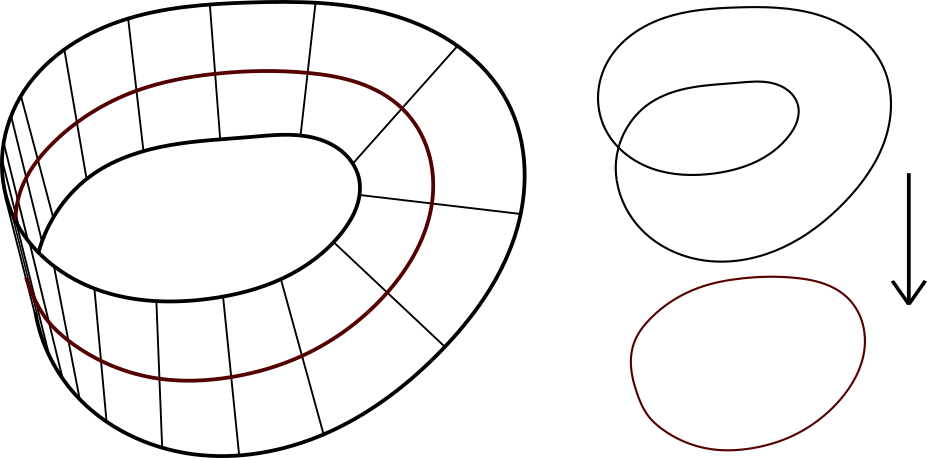
\includegraphics[width=.8\textwidth]{img/moebius.png}
    \caption{The Möbius-bundle over $S^1$ giving rise to a nontrivial covering over $S^1$ by assigning to each fiber the two possible orientations of that fiber.}\label{fig:moeb}
\end{figure}
The space $\BSO(n)$ classifies oriented vector bundles of rank $n$. Let $\t_n$ be the map $\BSO(n) \to \BO(n)$ which by postcomposition forgets orientation.
A lift of an orientable vectorbundle $V$ (represented by a map $M\to \BO(n)$) along $\t_n$ corresponds precicely to a choice of orientation for $V$. 
The map $\t_n$ is a partial double cover, since there are always exactly two possible orientations for a given orientable bundle.
The family of Maps $\t_n$ is compatible with stabilization, for this we just fix the usual orientation $\R^k$ to be the orientation of any trivial bundle. 
Therefore we obtain a colimit map $\t\colon \BSO \to \BO$ which by abstract nonsense is a fibration.\\
The tuple $(\BSO,\t)$ is now a tangential structure by above definition. 
A manifold $M$ admits this $\t$-structure, if its stable tangent bundle lifts along $\t$, i.~e. for some $K\in\N$ and all $k\geq K$ the $k$-times stabilized tangent bundle $TM\oplus \epsilon_k$ is orientable.
It is an elementary fact that $\mathfrak{o}(TM\oplus \epsilon_k) \to M$ is just the usual orientation double cover of $M$, so the choice of an orientation for $M$ makes up exactly to the choice of an orientation for some (and then all) $TM\oplus\epsilon_k$.
The example shows, that for $\t\colon \BSO \to \BO$ a manifold $M$ has a $\t$-structure if and only if it is orientable, and a $\t$-manifold is hence just a oriented manifold. \\
A more systematic way of obtaining interesting examples of $\theta$-structures comes from the \emph{Whitehead-tower} of $\BO$.
We denote it by 
\begin{equation*}
    \cdots \to \BO\langle k\rangle \to \cdots \to \BO\langle 2\rangle \to \BO\langle 1\rangle \to \BO\langle 0\rangle = \BO.
\end{equation*}
All the horizontal maps are fibrations, and the $k$-th stage is obtained from the one below by attaching cells killing the $k$-th homotopy group.
\begin{figure}
    \centering
    \includegraphics[width=\textwidth]{img/tikz/bott.pdf}
    \caption{Homotopy groups of $\BO,\BSO$, and $\BSpin$}\label{fig:bott}
\end{figure}
Due to the celebrated Bott periodicity theorem, the homotopy groups of the stable orthogonal group $\mathrm{O}$ are known and $8$-periodic (see \fref{fig:bott}).
From these, one obtains the homotopy groups of $\BO$ using the loopspace-suspension adjuncion in
\begin{equation*}
    \pi_{i+1}(\BO) = [S^{i+1},\BO] \cong [\Sigma S^i,\BO] \cong [S^i,\Omega\BO] \cong [S^i,\mathrm{O}] = \pi_i(O)
\end{equation*}
as well as the fact that $\B$ is a delooping.
The space $\BO$ has thus just the homotopy groups of $\mathrm{O}$ shifted up by one (see again \fref{fig:bott}), and is furthermore pathconnected.
Lifting a map, say the stable tangent bundle of a manifold, up by a stage is possible if the lifting obstructions for that stage vanishes.
We will take some time to elaborate that point and see how this construction generalizes the example of oriented bundles.
The fiber of the $k$-th fibration $\BO\langle k \rangle \to \BO\langle k -1 \rangle$ is an \emph{Eilenberg--MacLane-space} for the group $\pi_{k}(\BO)$ in degree $k$, which we denote $K(\pi_k(\BO),k)$ as is common.
Let $M$ be a manifold and $\hat{\st}\colon M\to \BO\langle k-1 \rangle$ a given lift of the stable tangent bundle, which we wish to lift one stage higher.
Denote by $M^{(i)}$ the $i$-skeleton of a CW-Decomposition of $M$, which since every smooth manifold admits a triangulation always exists.
We now wish to inductively solve the skeletal lifting problem
\begin{center}
    \begin{tikzcd}
        M^{(i+1)} \arrow[r, dashed] & \BO\langle k \rangle\arrow[d] \\
        M^{(i)} \arrow[u,hook]\arrow[ur]\arrow[r,"\hat{\st}"] & \BO\langle k-1 \rangle
    \end{tikzcd}
\end{center}
that asks whether we can extend the given lift on the $i$-skeleton to the $i+1$-skeleton.
Since the Fiber $K\big(\pi_k(\BO),k\big)$ is $k-1$-connected, there are no obstructions up until the $k-1$-skeleton of $M$.
The lifting obstruction from the $k-1$ to the $k$-skeleton is given by a certain cohomology class 
\begin{equation*}
    c\in H^{k}\Big(\BO\langle k -1 \rangle;\pi_k\big(K(\pi_k(\BO),k)\big)\Big) = H^{k}\big(\BO\langle k-1 \rangle;\pi_k(\BO)\big)
\end{equation*}
If then $\hat{\st}^\ast c$ vanishes, we obtain a lift to the $k$-skeleton of $M$. 
All higher homotopy groups of the fiber vanish, so from there on no further obstructions arise, and we get the desired lift on $M$.
Since Eilenberg--MacLane-spaces represent cohomology, we can alternatively think of the single obstruction $c$ as a (homotopy class of) map $\BO\langle k-1 \rangle \to K\big(\pi_k(\BO),k\big)$, which we will also denote $c$ in slight abuse of notation.
The dashed lift in
\begin{center}
    \begin{tikzcd}
        & \BO\langle k\rangle \arrow[d] & \\
        M \arrow[r,"\hat{\st}"]\arrow[ur,dashed] & \BO\langle k -1\rangle \arrow[r,"c"] & K\big(\pi_k(\BO),k\big)
    \end{tikzcd}
\end{center}
then exists, if and only of $\pi_k(c\circ\tau) = 0$.
We will jump frequently between these two viewpoints of the lifting obstruction in this work.
How does the Whitehead-tower tie into the discussed example?
Since $\pi_1(\BO)\cong \zz$ and $\BSO$ is pathconnected, the double cover $\BSO \to \BO$ is already the universal cover $\BO\langle 1 \rangle \to \BO$.
We have $H^1(\BO;\zz) \cong \zz$ by Hurewicz and excision, so the first universal Stiefel--Whitney-class $\overline{w}_1$ provides the unique obstruction class to orientability.
Similarly, the second universal Stiefel--Whitney-class $\overline{w}_2\in H^2(\BSO;\zz) = H^2(\BO;\zz) \cong \zz$ is the unique lifting obstruction against $\BO\langle 2 \rangle \to \BSO$.
\begin{defi}[Spin]
    A spin-structure on a manifold is a $\theta$-structure for the fibration $\t\colon \BSpin = \BO\langle 2\rangle \to \BO$. We call the $\theta$-manifolds of this tangential structure spin-manifolds.
\end{defi}
By the above, a manifold $M$ with stable tangent bundle $\st\colon M \to \BO$ is therefore orientable, iff $w_1(TM) = \st^\ast \overline{w}_1$ vanishes and \emph{spinnable} iff furthermore $w_2(TM) = \st^\ast \overline{w}_2$ vanishes aswell.\\
A surface $S$ is orientable if and only if it contains no Moebius-band.
Can we generalize this intuition to higherdimensional manifolds?
And what does a Spin-structure even entail geometrically?
We finish this section with such a geometric interpretation, which will be directly extracted from the obstruction theory point of view above.
\begin{thesislemma}\label{geomspin}
Let $M$ be a manifold. Then $M$ is orientable, if and only if for any continuous $\iota\colon S^1 \to M$ the restriction $\st\circ \gamma$ of the stable tangent bundle is trivializable.
    If $\dim(M)\geq 3$, $M$ is furthermore spinnable, if and only if additionally for any surface $S$ and continuous map $\iota\colon S\to M$ the restriction $\st\circ \iota$ is trivializable. 
\end{thesislemma}
\pagebreak{} % ugly but neccesary, for some reason prf sticks to lem
\prf
    Let $[X]\in H_d(X;\zz)$ denote the $\zz$ fundamental class of a $d$-dimensional manifold $X$. 
    The family
    \begin{equation*}
        \big\{ \iota_\ast [S_i] \:\big\vert\: \iota\colon S_i \to M, S_i \text{ compact manifold of dim } i \big\}
    \end{equation*}
    obviously generates $H_i(M;\zz)$.
    We may thus test vanishing of the Stiefel--Whitney-classes of $M$ on this family.
    Via naturality
    \begin{equation*}
        \langle w_i(TM), \iota_\ast[S_i] \rangle = \langle \iota^\ast w_i(TM), [S_i] \rangle = \langle w_i(\iota^\ast TM),[S_i]\rangle 
    \end{equation*}
    so the $i$-th Stiefel Whitney class of $M$ vanishes if and only if it vanishes restricted along all $S_i \to M$.
    $[S^1,\BO]$ has only two elements, so vanishing of the first Stiefel--Whitney-class already implies trivializability of a bundle over $S^1$.
    This finishes the proof of the first part, since $S^1$ is the only one dimensional manifold.\\
    For the second part, note that it suffices looking at only orientable surfaces $S \to M$. 
    Any orientable rank $\geq 3$ bundle over a oriented surface is already trivial if its second Stiefel--Whitney-class vanishes.
    This is due to the following observation:
    Cutting out a disk $D\cong D^2$ from a surface $S$ we may retract the remains to a wedge of circles, the $1$-skeleton of $S$.
    Over this $1$-skeleton, the bundle trivializes due to the vanishing of $w_1$.
    Since $D\whe \{\ast\}$ also there the bundle trivializes and we thus obtain all rank $d$ vectorbundles over the surface by a clutching map $S^1 \to SO(d)$.
    Now for $d\geq 3$ we have $\pi_1(\mathrm{SO}(d)) \cong \pi_2(\BSO) \cong \zz$, so vanishing of $w_2$ implies trivializability.
\endprf
For manifolds of dimension $1$ the lemma of course holds vacuously, but in dimension $2$ the relationship is knavish.
Whilst the tangent bundle of $S^2$ is famously nontrivial due to the hairy-ball-theorem, it has trivial Stiefel--Whitney-classes, since embedding $S^2$ into $\R^3$ gives a decomposition $TS^2 \oplus \underline{\R} \to T\R^3$ where $\underline{\R} = S^2\times\R$ is the trivialized normal bundle of the embedding.
Hence $S^2$ is spinnable, but its tangent bundle pulled back along the identity is nontrivial, violating the lemma.
The violation is not severe however, any orientable surface $S$ is spinnable, since if its genus is larger than $0$, we have $\pi_2(S) = 0$ removing $w_2$.\\
To strenghten the geometrical picture further, we pass from arbitrary maps to embeddings.
\begin{thesisprop}\label{orgeom}
    Let $M$ be a manifold. Then $M$ is orientable if $\iota^\ast TM$ is trivial for every embedding $\iota\colon S^1 \to M$.
\end{thesisprop}
\prf
    For $\dim(M) = 1$, the statement is easily verified by taking $\id_{S^1}$ as the embedding.
    Else, note that the homotopy class of any map $f\colon S^1 \to M$ contains a smooth representative by the Whitney approximation theorem.
    With $\dim(M)\geq 3$, this smooth representative may be taken to be an embedding by the Whitney embedding theorem, and the proposition follows instantly from \ref{geomspin}.
    In dimension $2$, one can use the classification of surfaces to directly see that every nonorientable surface contains a Möbius-band.
\endprf
This is best visualized in the following example:
A half equator $S_+^1 \hookrightarrow S^2$ maps onto a $S^1 \hookrightarrow \RP^2$ under the canonical projection $S^2\to \RP^2$. 
The normal bundle $\nu$ of this embeddeding $\iota\colon S^1\hookrightarrow \RP^2$ is the nontrivial Moebius-bundle, and the tangent direction is trivial.
Thus in total the restriction of the tangent bundle of $\RP^2$ along $\iota$ has $w_1(\iota^\ast T\RP^2) = w_1(\nu) \neq 0$ showing that it is nontrivial and $\RP^2$ is nonorientable!
\begin{thesisprop}\label{moregeomspin}
    Let $M$ be a simply connected manifold of dimension $d\geq 5$. Then $M$ is spinnable, if $\iota^\ast TM$ is trivial for every embedding $\iota\colon S^2 \to M$.
\end{thesisprop}
\prf
    Since $M$ is simply connected, $w_1(M) = 0$ and by Hurewicz every element in $H_2(M)$ comes from a continuous map $S^2 \to M$.
    With $d\geq 5 = 2* 2 + 1$ we may again use the Whitney approximation and embedding theorem to deform any such continuous map to an embedding. 
    Then as another application of \ref{geomspin} the proof is done.
\endprf


\subsection{Tangential type of a manifold}
The last section discussed questions of the form: Given a tangential structure $\theta$, which manifolds carry a $\theta$-structure?
This section takes a glance in the opposite direction.
What is the \emph{most tangential structure} we can equip a given manifold with? 
This is answered by the following lesser known invariant.
\begin{defi}[Tangential $k$-type]
    Let $k$ be any positive integer, $(B,\t)$ a tangential structure and $M$ a $\t$-manifold. If both ...
    \begin{itemize}[noitemsep, label=$\dots$]
        \item $\t \colon B\to \BO$ is $k$-coconnected
        \item the lift of $M \to B$ of $\st_M$ is $k$-connected
    \end{itemize}
    the tangential structure $(B,\t)$ is called tangential $k$-type of $M$.
\end{defi}
We will denote the $k$-th stage in the \emph{Moore-Postnikov--factorization} of $\st\colon M \to \BO$ by 
\begin{center}
    \begin{tikzcd}[row sep=small]
        & B^k(M) \arrow[dr, "\t"] & \\
        M \arrow[rr, "\st"] \arrow[ur, "\st^k"] & & \BO. 
    \end{tikzcd}
\end{center}
Now $\t$ is indeed $k$-coconnected, a fibration, and $\st^k$ is $k$-connected, so we have succeeded in our attempt to prove existence of the tangential $k$-type. 
The next lemma concerns uniqueness.
\begin{thesislemma}\label{ttunique}
    If $(B,\t)$ and $(B^\prime,\t^\prime)$ are two tangential $k$-types of a manifold $M$, then there is a homotopy equivalence of fibrations $\t\whe\t^\prime$.
\end{thesislemma}
\prf
We need to construct a pair of homotopy equivalences $ r\colon B \to B^\prime$ and $l\colon B^\prime\to B$ that fit in a commuting diagram like
    \begin{center}
        \begin{tikzcd}[row sep=small]
            B \arrow[rr, transform canvas={yshift=.3ex}, "r"] \arrow[dr, swap, "\t"] & & B^\prime \arrow[ll, transform canvas={yshift=-.3ex}, "l"] \arrow[dl, "\t^\prime"]\\
            & \BO & 
        \end{tikzcd}
    \end{center}
This suggests that $r$ should be the lift of $\t$ along $\t^\prime$ and $l$ vice verca the lift of $\t^\prime$ along $\t$.
By the symmetry of the situation it suffices to detail the construction of $r$. 
%Let $B^{(i)}$ denote the $i$-skeleton of a CW-decomposition of $B$. 
%The $i$-th lifting obstruction for the skeletal lifting problem
%\begin{center}
    %\begin{tikzcd}
        %B^{(i+1)} \arrow[r, dashed, "r^{(i+1)}"] & B^\prime \arrow[d,"\theta^\prime"] \\
        %B^{(i)} \arrow[u,hook]\arrow[r, "\t"]\arrow[ur,"r^{(i)}"] & \BO
    %\end{tikzcd}
%\end{center}
%is a class in $H^{i+1}\big(\BO,\pi_i(\hofib (\theta^\prime))\big)$. 
%Since $\theta^\prime$ is $k$-coconnected, $\pi_i(\hofib (\theta^\prime)) = 0$ for $i \geq k$, and there arise no problems with lifting in this range.
%For $i< k$ any approach with obstruction theory is doomed, since one always needs $\pi_1(\BO)$ to act trivially on $\pi_i(B^\prime)$, a luxury that we can not hope to enjoy.
An approach with obstruction theory is doomed, since one needs $\pi_1(\BO)$ to act trivially on $\pi_i(\B^\prime)$ for this, a luxury that we cannot afford.
Therefore a more bare-bones argument is required.\\
It is a nifty change of perspective that does the trick:
Instead of extending the map $\theta$, in the following we view $B^\prime$ as a sort of subspace in $\BO$, and compress $\t$ down to this subspace.
The Map $\hat{\st}\colon M\to B$ is $k$-connected, so (after replacing $B$ with the mapping cylinder of $\hat{\st}$, which we may do up to equivalence of fibrations) we can view $(B,M)$ as a relative CW-complex made by only attaching cells of dimension $> k$. 
Similarly, since $\t^\prime$ is $k$-coconnected, we may view $\BO$ as being built from $B^\prime$ by attaching cells of dimension $\leq k$.
We now look at the map $(\t,\hat{\st}^\prime)\colon (B,M) \to (\BO,B^\prime)$ of relative CW-complexes. 
\begin{center}
    \begin{tikzcd}[row sep=tiny]
        B \arrow[r,"\t"]\arrow[ddr, dashed, "r"] & \BO\\
        \mathrm{Cyl}{(\hat{\st})} \arrow[draw=none]{u}[sloped,auto=false]{\whe} & \mathrm{Cyl}{(\t^\prime)} \arrow[draw=none]{u}[sloped,auto=false]{\whe}\\ 
        M \arrow[draw=none]{u}[sloped,auto=false]{\subseteq}\arrow[r,"\hat{\st}^\prime"] & B^\prime  \arrow[draw=none]{u}[sloped,auto=false]{\subseteq}
    \end{tikzcd}
\end{center}
And by what Hatcher calls the \emph{compression lemma} the dashed compression $r$ exists, if $\pi_i(\hofib(\t^\prime))$ vanishes in those degrees where we glued cells to $M$ to obain $B$, exactly what we have.
The map $r$ is homotopic to $\theta$ viewed as maps to $\mathrm{Cyl}(\theta^\prime)$, so it is $k$-coconnected.
Since the inclusion of $M$ into $\mathrm{Cyl}(\hat{\st})$ is $k$-connected and the diagram commutes, one easily also sees that $r$ must be $k$-connected.
Therefore $r$ is a weak homotopy equivalence, and by Whiteheads theorem even a homotopy equivalence.
\endprf
We have now established that the tangential $k$-type is indeed a well defined invariant of a manifold.
Let us compute the tangential $k$-type of the Sphere $S^d$ with $d>k$ first.
We have $\pi_i(S^d) = 0$ for $0<i<d$, so to admit a $k$-connected map $S^d \to B^k(S^d)$ we have to have $\pi_i(B^k(S^d)) = 0$ for $0<i\leq k$ aswell.
In colloquial terms we thus search for a space that looks like $\BO$ with killed lower $k$ homotopy groups. 
Such a space we find in the $k$-th stage of the Whitehead-tower of $\BO$. 
The lifting obstruction of the stable tangent bundle $\st\colon S^d \to \BO$ for the $i$-th stage is given by the homotopy class of a map $S^d \to K(\pi_i(\BO),i)$, or equivalently an element in $\pi_d(K(\pi_i(\BO),i))$.
Since for $i\leq k <d$ we have $\pi_d(K(\pi_i(\BO),i))= 0$, the stable tangent bundle lifts to a $k$-connected map $S^d\to \BO\langle k \rangle$.
By construction $\BO\langle k \rangle \to \BO$ is $k$-coconnected, thus the example is concluded: $B^k(S^d) = \BO\langle k\rangle$ for $k<d$.\\
The main result of this chapter will be the classification of all tangential $2$-types. 
To prepare ourselfes, we begin with the easier classification of tangential $1$-types, which is closely related to the earlier example of orientable vector bundles.
\begin{thesisprop}
    Let $M$ be a connected manifold with first Stiefel Whitney class $w_1 = w_1(TM)\in H^1(M;\zz)$. Then the tangential $1$-type of $M$ is ...
    \begin{itemize}[noitemsep]
        \item[...] $(\BO,\id_\BO)$ if $w_1 \neq 0$.
        \item[...] $(\BSO, \BSO \to \BO)$ if $w_1 = 0$.
    \end{itemize}
\end{thesisprop}
\prf
    Both $\id_\BO$ and $\BSO\to\BO$ are $1$-coconnected, so all there is to study is the connectivity of $\st\colon M\to \BO$.
    Either $\pi_1(\st)$ is surjective, then $\st$ is already $1$-connected and the tangential type is $\id_\BO$, or $\pi_1(\st)$ not surjective, implying $\im(\pi_1(\st)) = \{0\}$ since $\pi_1(\BO) \cong \zz$. 
    In the second case $\st$ then lifts to a map into the universal cover $\BSO \to \BO$, which is trivially $1$-connected.\\
    To connect the Stiefel Whitney class with the vanishing of the homeomorphism $\pi_1(\st)$ we first use the fact that $\pi_1(\BO)= \zz$ is abelian to descend via Hurewicz to the map $\st_\ast$ on $H_1$.
    Using Universal Coefficients we get 
    \begin{center}
        \begin{tikzcd}[row sep=small]
            0 = \Ext_\Z^1(\Z,\zz) \arrow[r, ""] & H^1(M;\zz) \arrow[r, "\cong"] & \Hom_\Z(H_1(M;\Z),\zz) \\ 
            0 = \Ext_\Z^1(\Z,\zz) \arrow[r, ""] & H^1(\BO ;\zz) \arrow[r, "\cong"] \arrow[u, "\st^\ast"] & \Hom_\Z(H_1(\BO ;\Z),\zz ) \arrow[u, "\Hom(\bullet{,}\,\zz)( \st_\ast )"] 
        \end{tikzcd}
    \end{center}
    and so $\pi_1(\st)$ is the zero map if and only if $\st^\ast$ is the zero map. But since $\st^\ast(w_1(\BO)) = w_1$, this depends on whether $w_1 = 0$.
\endprf
Following is a rather involved computation of the possible tangential $2$-types of connected manifolds. 
The difficulty in comparison to above arises from the fundamental group of $M$ playing a much more pronounced role when we demand $M\to B^2(M)$ to be $2$-connected.
\begin{thesisprop}\label{tttypes}
    Let $M$ be a connected manifold with Fundamental group $G = \pi_1(M)$ first and second Stiefel Whitney classes $w_i = w_i(TM) \in H^i(M;\zz)$. 
    Denote the Universal Cover of $M$ by $\widetilde{M}$ and the second Stiefel Whitney class of the Universal Cover by $\widetilde{w}_2 = w_2(T\widetilde{M}) \in H^2(\widetilde{M};\zz)$.
    Then we have six different families of tangential $2$-types, parametrized by $G$:
    \begin{enumerate}[noitemsep, label=\Roman*., labelindent=3cm, labelwidth=!]
        \item $ \widetilde{w}_2 \neq 0, w_1 \neq 0, w_2 \neq 0,\quad$ resulting in type $\BO \times_{\B \zz} \B G$,
        \item $ \widetilde{w}_2 \neq 0, w_1 = 0, w_2 \neq 0,\quad$ resulting in type $\BSO \times \B G$,
        \item[III. - VI.] $\widetilde{w}_2 = 0\quad\quad\quad\quad\quad\quad\quad\quad\,$ resulting in type $\B(G,w_1,w_2)$.
    \end{enumerate}
    For the defining fibrations to $\BO$ and the definition of $\B(G,w_1,w_2)$ consult the proof.
\end{thesisprop}
The keen eye immeadiately recognizes there are two cases missing, namely those with $w_2 = 0$ but $\widetilde{w}_2 \neq 0$. 
While these are perfectly fine cases in the abstract construction below, they of course never appear as a tangential $2$-type:
The covering map $p\colon \widetilde{M} \to M$ gives a bundle map $T\widetilde{M} \to T M $ and thus by naturality $\widetilde{w}_2 = p^\ast w_2$. 
Therefore $w_2 = 0$ implies $\widetilde{w}_2 = 0$.
Before diving into the proof of \ref{tttypes}, we will first climb to a slightly higher outpost of abstraction to unify the approaches instead of handeling all six cases separately.
\begin{defi}[Tangential datum]
    Let $G$ be a group. A tangential datum over $G$ is an equivalence class of triples $(G,w_1,w_2)$ where $w_i \in H^i(\B G ;\zz)$. Two such triples $(G,w_1,w_2)$ and $(G^\prime, w_1^\prime, w_2^\prime)$ are called equivalent if there exists an Isomorphism $\phi\colon G \to G^\prime$ with $\phi^\ast w_i^\prime = w_i$.
\end{defi}
A manifold $M$ gives rise to (parts of) a tangential datum as follows: 
To noones surprise, set $G = \pi_1(M)$.
We may think of the univeral cover as being classified by a $2$-connected Map $u\colon M \to \B G$.
Notice how by Hurewicz and Universal coefficients then also $u^\ast\colon H^1(\B G;\zz) \to H^1(M;\zz)$ is an isomorphism.
Therefore we have a unique class $w_1 \in H^1(\B G,\zz)$ with $u^\ast w_1 = w_1(M)$.\\
In the case that $w_2(\widetilde{M}) = p^\ast w_2(M) = 0$ we use the exact sequence 
\begin{equation*}\tag{$\heartsuit$}\label{heartseq}
    0 \to H^2(\B G ; \zz) \overset{u^\ast}{\to} H^2(M;\zz) \overset{p^\ast}{\to} H^2(\widetilde{M}) \cdots
\end{equation*}
to similarly obtain a unique class $w_2 \in H^1(\B G,\zz)$ with $u^\ast w_2 = w_2(M)$. 
Otherwise, if $w_2(\widetilde{M})\neq 0$, the statement and discussion of \ref{tttypes} suggest we will not need any further information than $w_1$, and the proof will underpin this.\\
The sequence $\heartsuit$ comes from a slightly involved argument, which \cite{kreck:sad} attributes to \cite{brown:cog}. 
For sake of accessibility, the argument shall be expanded here.
Up to replacing $M$ and $\widetilde{M}$ by weakly homotopy equivalent spaces, the classifying map of the universal cover $u$ gives rise to a fibration sequence
\begin{equation*}
    \widetilde{M} \fib M \overset{u}{\to} \B G.
\end{equation*}
From the Atiyah--Hirzebruch spectral sequence $E^{p,q}$ of this fibration with $\zz$ coefficients we observe (see \fref{fig:ahss}) the following facts, using constantly that $H^1(\widetilde{M},\zz) = 0$ and thus $E_2^{q,1} = 0$ for all $q\in\N$.
\begin{enumerate}[label=(\roman*)]
    \item The second cohomology of $\B G$ at $E_2^{2,0}$ is not hit by any nontrivial differentials, hence we have $H^2 (\B G; \zz) = E_2^{2,0} = E_\infty^{2,0}$.
    \item The second cohomology of $\widetilde{M}$ at $E_2^{0,2} = E_3^{0,2}$ admits a single nontrivial differential to $E_3^{3,0}$, which we call $d_3$. Then $E_\infty^{0,2} = E_4^{0,2} = \ker(d_3) \subset E_3^{0,2} = H^2(\widetilde{M},\zz)$.
    \item Since we have field coefficients, we compute the second cohomology of $M$ as $H^2(M;\zz) \cong E_\infty^{0,2} \oplus E_\infty^{1,1}\oplus E_\infty^{2,0} = \ker(d_3) \oplus H^2(\B G,\zz)$.
\end{enumerate}
\begin{figure}
    \centering
    \includegraphics[width=.48\textwidth]{img/tikz/e2.pdf}
    \includegraphics[width=.48\textwidth]{img/tikz/e_infty.pdf}
    \caption{The $E_2$ page (left) and $E_\infty$ page (right) in the Atiyah--Hirzebruch spectral sequence of $u$.}\label{fig:ahss}
\end{figure}
By including into and projecting from the direct sum in (iii) to its components, we obtain a sequence
\begin{equation*}
    0 \to H^2(\B G;\zz) = E_\infty^{2,0} \hookrightarrow H^2(M;\zz) \cong \ker(d_3) \oplus H^2(\B G;\zz) \to \ker(d_3) \hookrightarrow H^2(\widetilde{M};\zz).
\end{equation*}
This sequence is the desired sequence $\heartsuit$.
exactness at $H^2(\B G;\zz)$ is obvious, as it just amounts to the Injectivity of the inclusion Map.
Due to the monomorphism property of the last Map, the exactness of $\heartsuit$ at $H^2(M;\zz)$ is ruled by the evident exactness of the above sequence at the Direct Sum.\\
The only caveat left is the identification of the composite $H^2(M;\zz) \to \ker(d_3) \to H^2(\widetilde{M};\zz)$ with $p^\ast$.
This fact is a not something specific to this case, but rather a general fact of the Atiyah--Hirezebruch-sequence of a fibration.
A proof can be for example found as the proof of theorem 5.~9 in \cite{mc:guide}.
After this digression to the world of spectral sequence calculations, we are finally ready to prove \ref{tttypes}.\\
\prf
    We will digest the cases in the order they appear in the proposition.\\
    \textbf{I.} As a quick warmup, let us handle the first case $w_2(\widetilde{M}) \neq 0$ and $w_1(M) \neq 0$. 
    Begin by obtaining $(G,w_1)$ as illustrated above.
    Let $\overline{w}_1\in H^1(\BO; \zz)$ denote the first universal Stiefel--Whitney-class.
    Since $\B\zz$ is an Eilenberg--MacLane-space $K(\zz, 1)$ We may think of $\overline{w}_1$ as being represented by a map $\BO \to \B\zz$, which we name $\overline{w}_1$ by slight abuse of notation.
    The square
    \begin{center}
        \begin{tikzcd}
            M \arrow[r,"u"]\arrow[d,"\st"] & \B G \arrow[d,"w_1"] \\
            \BO \arrow[r,"\overline{w}_1"] & \B\zz 
        \end{tikzcd}
    \end{center}
    commutes, since $\st^\ast \overline{w}_1 = w_1(TM) = u^\ast w_1$ by definition.
    We therefore get a well defined map $\hat{\st}$ to the pullback which is a lift of $\st$ along $\theta$.
    \begin{center}
        \begin{tikzcd}
             & \BO\times_{\B\zz}\B G \arrow[r]\arrow[d,"\theta"] & \B G \arrow[d,"w_1"] \\
            M \arrow[r,"\st"] \arrow[dashed, ur,"\hat{\st}"] & \BO \arrow[r,"\overline{w}_1"] & \B\zz 
        \end{tikzcd}
    \end{center}
    Replacing $\B G$ with a weakly equivalent space, we may assume that $w_1$ is a fibration.
    Hence the pullback above is a homotopy pullback and we have $\pi_i(\hofib (\theta)) \cong \pi_i(\hofib (w_1))$.
    The latter vanishes for $i\geq 2$, as $\pi_i(\B\zz) \cong 0 \cong \pi_i(\B G)$ for $i\geq 2$ and we have the LES of $w_1$:
    \begin{equation*}
        \cdots \to \pi_{i+1}(\B\zz) \to \pi_i(\hofib (w_1)) \to \pi_i(\B G) \to \cdots
    \end{equation*}
    We conclude, that the map $\theta$ is indeed $2$-coconnected.\\
    Comparing the two long exact sequences of the vertical fibrations $\theta$ and $w_1$ we obtain
    \begin{center}
        \begin{tikzcd}[column sep=small]
            \pi_2(\BO) \arrow[r]\arrow[d] & \pi_1(\hofib (\theta)\arrow[r]\arrow[d,"\cong"] & \pi_1(\BO \times_{\B\zz} \B G) \arrow[r,"{\pi_1(\theta)}"]\arrow[d,"r"] & \pi_1(\BO) \arrow[r]\arrow[d,"{\pi_1(\overline{w}_1)}"] & \pi_0(\hofib(\theta)) \arrow[d,"\cong"] \\
            0 = \pi_2(\B\zz) \arrow[r] & \pi_1(\hofib (w_1)) \arrow[r] & \pi_1(\B G) \arrow[r,"{\pi_1(w_1)}"] & \pi_1(\B\zz) \arrow[r] & \pi_0(\hofib(w_1)).
        \end{tikzcd}
    \end{center}
    The homeomorphism $\pi_1(\overline{w}_1)$ is nontrivial and since $\pi_1(\BO) \cong \zz$ also an isomorphism. 
    The $5$-lemma thus gives the ratiocination that $\pi_1(\BO\times_{\B\zz} \B G) \cong G$.
    Since the isomorphism $\pi_1(u)$ factors over $\pi_1(\BO\times_{\B\zz}\B G)$ in 
    \begin{center}
        \begin{tikzcd}
            M \arrow[d,"\hat{\st}"] \arrow[dr, "u"] & \\
            \BO\times_{\B\zz}\B G \arrow[r] & \B G 
        \end{tikzcd}
    \end{center}
    we can conclude that $\pi_1(\hat{\st})$ is an isomorphism by the two--out--of--three-property.
    Note that $\pi_2(\BO\times_{\B\zz}\B G) \cong \pi_2(\BO) \cong \zz$ from consultation with the LES of the horizontal maps in the pullback diagram and $5$-lemma.
    Hence for showing that $\pi_2(\hat{\st})$ is an epimorphism, it is sufficient to show that $\pi_2(\st)$ is an epimorphism.
    Since $w_2(\widetilde{M}) \neq 0$, the classifying map of the stable tangent bundle of $\widetilde{M}$ is an epimorphism onto $\pi_2(\BO)$.
    It factors as $\st\circ p$, since $p$ is a local diffeomorphism, so therefore also $\st$ is an epimorphism on $\pi_2$, concluding the argument that $\hat{\st}$ is $2$-connected.\\ 
    \textbf{II.} In the case $w_2(\widetilde{M}) \neq 0$ and $w_1(M) = 0$, the composition of fibrations
    \begin{equation*}
        \theta\colon \B G \times \BSO \overset{\mathrm{pr}}{\to} \BSO \overset{t}{\to} \BO
    \end{equation*}
    is the tangential type of $M$, where $t\colon \BSO \to \BO$ is the universal covering map.
    Since $M$ is orientable, the stable tangent bundle of $M$ lifts along $t$ to a oriented bundle $\hat{\st} \colon M \to \BSO$.
    The lift of $\st$ along $\theta$ is now given by the tuple $(u,\hat{\st})$, where $u\colon M \to \B G$ as always denotes the classifying map of the universal cover $p\colon \widetilde{M} \to M$.\\
    The fiber $\B G$ of the projection $\mathrm{pr}$ is $2$-coconnected, so $\mathrm{pr}$ is $2$-coconnected.
    Similarly, also $t$ is as a covering map $2$-coconnected, and by composition therefore $\theta$ is $2$-coconnected.
    As we know, the map $u$ is an isomorphism on $\pi_1$, and since $\pi_1(\BSO) = 0$, this makes $(u,\hat{\st})$ an isomorphism on $\pi_1$.
    On the level of $\pi_2$, the complementary situation arises:\\
    With $\pi_2(\B G) = 0$ the homeomorphism $\pi_2((u,\hat{\st}))$ is completely determined by $\pi_2(\hat{\st})$.
    A similar idea as in case I now applies.
    An orientation of $\st$ fixes a compatible orientation of the stable tangent bundle of $\widetilde{M}$.
    We may thus think of the stable tangent bundle of the universal cover of $M$ as a map $\widetilde{\st}\colon\widetilde{M} \to \BSO$ that satisfies $\widetilde{\st} = \hat{\st}\circ p$.
    Again, $\pi_2(\widetilde{\st})$ may not be the trivial map, for else $w_2(\widetilde{M})$ was trivial.
    Since $\pi_2(\BSO) \cong \zz$, this immediately implies surjectivity of $\pi_2(\widetilde{\st})$.
    And again by the same argument as in case I we obtain surjectivity of $\pi_2(\hat{\st})$ as a consequence.\\
    \textbf{III.- VI.}
    In the case $w_2(\widetilde{M})= 0$ first obtain a tangential datum $(G,w_1,w_2)$ from $M$.
    We again want to think of $w_i\in H^i(\B G; \zz)$ as being represented by maps to the according Eilenberg--MacLane-space $w_i \colon \B G \to K(\zz,i)$.
    We also consider the universal Stiefel--Whitney-classes $\overline{w}_i\in H^i(\BO;\zz)$ as being represented by such maps.
    For readability we introduce the notation $\B^2\zz$ for $K(\zz ,2)$.
    Replace again $\B G$ by a weakly equivalent space such tha t $(w_1,w_2)\colon \B G \to \B \zz \times \B^2 \zz$ becomes a fibration.
    Then for the same reason as in the warmup case the square
    \begin{center}
        \begin{tikzcd}
            M \arrow[r,"u"]\arrow[d,"\st"] & \B G \arrow[d,"{(w_1,w_2)}"] \\
            \BO \arrow[r,"{(\overline{w}_1,\overline{w}_2)}"] & \B \zz \times \B^2 \zz
        \end{tikzcd}
    \end{center}
   commutes, and we get a well defined lift $\hat{\st}$ along the fibration $\theta$ in the (homotopy) pullback
    \begin{center}
        \begin{tikzcd}
            & \B (G,w_1,w_2) \arrow[r]\arrow[d,"\theta"] & \B G \arrow[d,"{(w_1,w_2)}"] \\
            M \arrow[r,"\st"] \arrow[dashed, ur,"\hat{\st}"] & \BO \arrow[r,"{(\overline{w}_1,\overline{w}_2)}"] & \B \zz \times \B^2 \zz
        \end{tikzcd}
    \end{center}
    Analogous to the first case we use the LES of the fibration $(w_1,w_2)$ together with the observation that $\pi_i(\B G) = 0$ for $i\geq 2$ and $\pi_i(\B\zz \times \B^2\zz) = 0$ for $i\geq 3$ to compute that for $i\geq 2$ we have $\pi_i(\hofib(\theta))\cong \pi_i(\hofib((w_1,w_2))) \cong 0 $.
    We thus establish that $\theta$ is $2$-coconnected.\\
    Turning our eye towars the analysis of $\hat{\st}$ we first notice, that again due to the commutativity of 
    \begin{center}
        \begin{tikzcd}
            M \arrow[d,"\hat{\st}"] \arrow[dr, "u"] & \\
            \B (G,w_1,w_2) \arrow[r] & \B G 
        \end{tikzcd}
    \end{center}
   we get injectivity of $\pi_1(\hat{\st})$ for free. 
   Writing down the $5$-lemma diagram from the vertical fibrations again and using that $\pi_i(\overline{w}_i)$ are isomorphisms, as in case I we see $\pi_1(\B(G,w_1,w_2)) \cong G$, so $\pi_1(\hat{\st})$ is an isomorphism.
   The only different part of the calculation compared to the first case concerns the surjectivity of $\pi_2(\hat{\st})$.
   It is trivially fulfilled since $\pi_2(\B(G,w_1,w_2)) = 0$ as one can infer with yet another invocation of the $5$-lemma for
    \begin{center}
        \begin{tikzcd}[column sep=small]
            0\arrow[r] & 0\arrow[r]\arrow[d,"\cong"] & \pi_2(\B(G, w_1,w_2)) \arrow[r,"{\pi_2(\theta)}"]\arrow[d] & \pi_2(\BO) \arrow[r]\arrow[d,"{(0,\pi_2(\overline{w}_2))}"] & \pi_1(\hofib(\theta)) \arrow[d,"\cong"] \\
            0\arrow[r] & 0 \arrow[r] & \pi_2(\B G) \arrow[r,"{\pi_2((w_1,w_2))}"] & \pi_2(\B\zz\times\B^2\zz) \arrow[r] & \pi_1(\hofib((w_1,w_2)))
        \end{tikzcd}
    \end{center}
    with noting $\pi_2(\B G) = 0$.
    This concludes the computation of the possible tangential $2$-types of manifolds.
\endprf
As a remark, let us more explicitly determine the space $\B(G,0,0)$. 
If $M$ has vanishing $w_1$ and $w_2$, the stable tangent bundle $\st$ lifts along the $2$-coconnected fibration $\BSpin \to\BO$ from the Whitehead-tower.
The universal cover together with this lift form a map $M\to \BSpin \times \B G$ which is $2$-connected by an argument analogous to the argument in the second case of the proof.
By uniqueness (\ref{ttunique}), we get that the tangential $2$-type $\B(G,0,0)$ is just $\theta\colon \BSpin\times\B G \overset{\mathrm{pr}}{\to} \BSpin \to \BO$.\\
As a first application of the proposition, let us compute the tangential $2$-type of the real projective space $\RP^m$ for $m>1$.
We remind ourselfes, that the total Stiefel--Whitney-class of $\RP^m$ is given by $w= (1+c)^{m+1}$, where $c$ is a nontrivial element of degree $1$ representing the tautological bundle, subject only to the obvious relation $c^{m+1} = 0$.
The binomial theorem hands us
\begin{equation*}
    w_1(\RP^m) = (m+1)c,\quad w_2(\RP^m) = \begin{pmatrix} m+1 \\ 2 \end{pmatrix}c^2
\end{equation*}
and we immediately recognize the well known fact that $\RP^m$ is orientable if and only if $m$ is odd.
The analysis of $w_2$ is mildly laborious.
First notice, that the parity of the binomial coefficient in this case only depends on the remainder of $m$ dividing by $4$, since generally 
\begin{equation*}\tag{$\diamondsuit$}
    \begin{pmatrix} i\\2 \end{pmatrix} \mod 2 \equiv \begin{cases} 0 & i \equiv 0,1 \mod 4 \\ 1 & i\equiv 2,3 \mod 4.\end{cases}
\end{equation*}
Combining this with our knowledge that the universal cover $S^m$ of $\RP^m$ is always spinnable, and the fact that $\pi_1(\RP^m) \cong \zz$, we have as possible tangential types of the real projective spaces
\begin{center}\vspace{.5\baselineskip}
    \begin{tabular}{c|c|c|c|c}\hline\hline
        $m \mod 4$ & $0$ & $1$ & $2$ & $3$\\\hline
        $w_1(\RP^m) $ & $c$ & $0$ & $c$ & $0$\\
        $w_2(\RP^m) $ & $0$ & $c^2$ & $c^2$ & $0$\\
        Type & $\B(\zz,w_1,0)$ & $\B(\zz,0,w_2)$ & $\B(\zz,w_1,w_2)$ & $\BSpin\times\B\zz$ \\\hline\hline
    \end{tabular}\vspace{.5\baselineskip}
\end{center}
We now conclude this chapter with a bigger list of examples for each tangential type family.\\
 \textbf{I.} The $\BO\times\B G$ type family is for example inhabited by manifolds like $\RP^m\times\CP^n$ for $n,m\neq 0$ even.
        With $\RP^m$ being nonorientable for even $m$, so is the product, thus $w_1\neq 0$.
        For $w_2$, consult the Whitney product theorem to compute
        \begin{equation*}
                w_2(\RP^m\times\CP^n) = w_2(\RP^m) + w_1(\RP^m)w_1(\CP^n) + w_2(\CP^n),
        \end{equation*}
        where we disregard in our notation the obvious pullbacks along the canonical projections which make above formula welldefined.
        The total Stiefel--Whitney-class of $\CP^n$ is given by $(1+d)^{n+1}$ where $d$ is a degree $2$ element subject only to the relation $d^{n+1}= 0$.
        The binomial theorem now computes
        \begin{equation*}
                w_2(\CP^n) = (n+1)d
        \end{equation*}
        So indeed the $w_2(\CP^n) \neq 0$ iff $n$ even.
        The universal cover of $\RP^m\times\CP^n$ is given by $S^m\times\CP^n$.
        Since all Stiefel--Whitney-classes of $S^m$ vanish, by the Whitney product theorem we have $w_2(S^m\times\CP^n) = w_2(\CP^n)$ which is nonzero for $n$ even.\\
\textbf{II.} In the $\BSO\times \B G$ type family of manifolds we have the even complex projective spaces $\CP^{2n}$, as they are orientable  and have nonvanishing $w_2$ by above. 
        They are furthermore simply connected, which one sees nicely by the LES of the fibration sequence $S^1 \fib S^{2n+1} \to \CP^n$.
        Hence they are their own universal cover, so their universal cover isnt spinnable aswell.\\
\textbf{III.} In the $\BSpin\times\B G \to \BO$ type family we have with $G$ trivial all manifolds that satisfy the condition in \ref{moregeomspin}, as well as all spheres $S^d$ with $d>2$ and the odd complex projective spaces $\CP^{2n+1}$.
        Examples of manifolds with nontrivial fundamental group in this type family are given by $S^1$ and, more generally, all Tori since they are parallelizable.
        Furthermore all orientable $3$-manifolds are parallelizable, see \emph{Satz 21} in \cite{stiefel:cc} for the historical proof of this marvellous fact, and thus also belong to this family.
        Lastly, also in dimensions $1$ and $2$, all orientable manifolds are spinnable as we have discussed.\\
\textbf{I.-VI.} The \hypertarget{doldmnf}{\emph{Dold-manifolds}} $P(m,n)$ with odd $n$ provide more excellent examples in the type familes $\B(G,w_1,w_2)$.
        Define $P(m,n) = S^m\times\CP^n /_\sim$ where $(x,z) \sim (-x,\overline{z})$, a manifold with universal (double) cover $S^m\times\CP^n$ for $m>1$.
        By example I, their universal cover is thus spin exactly when $n$ is odd. 
        The total Stiefel--Whitney class of $P(m,n)$ is given by $w = (1+c)^m(1+c+d)^{n+1}$, where $c,d$ are nontrivial elements of degrees $1$ and $2$ (originally calculated by \cite{dold:bord}).
        It is straightaway computed that we get $ w_1(P(m,n)) = (n + m + 1)c$  vanishes iff $n$ and $m$ do not have the same parity.
        For the second Stiefel--Whitney-class we obtain
        \begin{equation*}
                w_2(P(m,n)) = (n+1)d + \left(\begin{pmatrix} m\\ 2 \end{pmatrix} + \begin{pmatrix} n +1 \\ 2\end{pmatrix} + (n+1)m\right)c^2.
        \end{equation*}
        Now remembering again identity $\diamondsuit$, there are only eight cases to consider, since we already fixed $n$ to be odd.
        \begin{sidewaysfigure}
            \centering
            \includegraphics[width=\textwidth]{img/tikz/pmn.pdf}
            \caption{The tangential type of the Dold manifolds $P(m,n)$ for varying $n>0$ and $m>1$. The symbol $/$ stands for a vanishing Stiefel--Whitney-class.}\label{fig:pmn}
        \end{sidewaysfigure}
        All these cases can found in the table in \fref{fig:pmn}, together with the cases for even $n$ giving tangential types I and II. \\

\clearpage

% Chapter 2
\section{Bordism with extra structure}\label{sec:bordism}
This chapter will deal with the theory of bordism, sometimes called cobordism in the literature.
We will begin by introducting a notion of $\t$-bordism, where $\t$ denotes a tangential structure as in the previous chapter.
The original and classical reference for this is \cite{stong:cc}.
Since we refrain from introducing bordism categories for the benefit of a more streamlined journey towards our goals, it may look like we diverge conciderably from the above book.
This is an illusion, as the core arguments stay precicely the same.
However, an even more similar approach to ours is presented in the survey \cite{milnor:bord}.\\
The \hyperlink{subsection.2.2}{second part of the chapter} then focuses on the flavour of bordism ($\id_\BO$-bordism) we need for the results in \hyperref[sec:psc]{the third chapter}. 
Since it is mostly a historic tour of the many wonders of unoriented bordism, the abundance of literature is woven into the fabric of the story and ought not to be repeated here.
We finish the second half explicitly calculating a set of additive generators of the unoriented bordism ring $\NN_\ast$, which will be of crucial importance for \hyperlink{subsection.3.2}{the proof of our main theorem}.

\subsection{Bordism of $\t$-Manifolds}
Bordism is an elementary concept: 
It introduces an equivalence relation on Manifolds, that calls two manifolds the same (alias \emph{bordant}) if their union in some sense arises as the common boundary of a third manifold (the \emph{bordism}) .
Making this precise and formulating a notion of $\t$-bordism compatible with a $\t$-structure, we need to explain how a $\t$-Structure on a manifold $M$ induces a $\t$-Structure on its boundary. 
Not every submanifold inherits the $\t$-structure from its surrounding.
There is for example an embedded equatorial $\RP^2 \hookrightarrow \RP^3$, and as we have seen $\RP^3$ is orientable and thus carries a $\BSO\to\BO$-strucure, while $\RP^2$ does not. 
The problem here was, that the normal bundle of $\RP^2 \subset \RP^3$ is nontrivial.
Removing this problem, one has the desired
\begin{thesislemma}
Let $(B,\t)$ denote a tangential structure and $M$ be a $\t$-Manifold of dimension $d$. 
Let $\iota\colon M^\prime \hookrightarrow M$ be an embedding of a $d^\prime \leq d$ dimensional manifold $M$ with trivial normal bundle $\nu$.
Then $M^\prime$ obtains an induced $\t$-structure.
\end{thesislemma}
\prf
By choice of a trivialization of $\nu$, we have $\iota^\ast TM= \nu \oplus TM^\prime \cong \underline{\R^k}\oplus TM^\prime$, so the $\t$-structure on $M^\prime$ induces one on $M$.
\endprf
A $\t$-structure on the target $M$ of a diffeomorphism $\phi \colon M^\prime \to M$ canonically induces a $\t$-structure on $M^\prime$ by the lemma, since the normal bundle has rank zero and is therefore trivial without any choice involved.
We call a diffeomorphism of $\t$-manifolds $\t$-preserving, if its induced $\t$-structure matches the given one.
Using the lemma, a decomposition $M = M_1 \amalg M_2$ also induces canonical $\t$-Structures on the components $M_i$, again $M_i \hookrightarrow M$ has rank zero normal bundle.
Already in the case of the boundary $\partial M\hookrightarrow M$ there is a choice involved. 
We fix this choice once and for all.
\begin{defi}[Boundary $\t$-structure]
    Let $M$ be a $\t$-Manifold with boundary $\partial M$.
    Then there is a unique $\t$-structure on $\partial M$ corresponding to the inner normal direction, which we call \emph{the} induced $\t$-structure on $\partial M$.
\end{defi}
The collar neighbourhood theoreom shows, that the normal bundle of $\partial M \hookrightarrow M$ is trivial, hence the lemma applies. 
There are two choices of trivializations given by the inner and outer normal field, possibly leading to two different lifts of the stable tangent bundle.
Choosing the inner normal field by convention, the lift becomes unique.
To see the phenomenon of nonuniqueness appear, consider a cylinder as in \fref{fig:cyl}. 
\begin{figure}
    \centering
    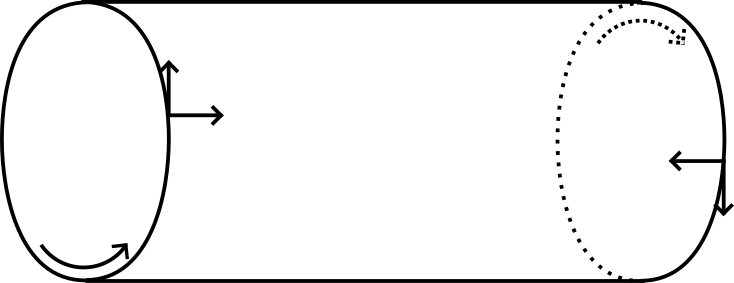
\includegraphics[width=.6\textwidth]{img/cyl.png}
    \caption{The cylinder $S^1\times [0,1]$ with boundary orientations induced by the inner normal direction.}\label{fig:cyl}
\end{figure}
Both boundary components of the cylinder are a circle, which we consider a $\BSO\to\BO$-manifold for this example. 
Picking the outer normal to induce the boundary orientations would have exactly switched the induced orientations on the two circles.\\
There is another subtle phenomenon which is illuminated by this cylinder:
Note how picking the inwards normal direction on both sides induces different orientations on the two circles.
If we were to define a bordism $M\bord M^\prime$ na\"{i}vely as a manifold with boundary $M\amalg M^\prime$, the resulting equivalence relation would have no reason to be reflexive, as the cylinder $M\times [0,1]$ in the oriented case would not define a bordism $M\bord M$.
This subtlety leads to the following defininition, artificially fixing the reflexivity problem.
\begin{defi}[Opposite manifold]
    Let $M\times[0,1]$ be a $\t$-Manifold. Then we call $M\times\{1\}$ and $M\times\{0\}$ with the induced boundary $\t$-structures opposites, and denote $M\times\{1\}$ with $-M\times\{0\}$ and vice versa. 
\end{defi}
By the path lifting property for fibrations, any $\t$-structure on $M\cong M\times\{0\}$ determines uniquely a $\t$-structure on $M\times[0,1]$, so every $\t$-manifold $M$ has an opposite $-M$.
As an example, again look at \fref{fig:cyl}, to see that as $\BSO \to \BO$-manifolds the opposite of $S^1$ oriented counterclockwise is $S^1$ oriented clockwise.
Moreover, we can forget orientation and see that as $\id_\BO$-manifolds the opposite of $S^1$, or any manifold for that sake, is just $S^1$.
\begin{defi}[$\t$-bordism]
    Let $M,M^\prime$ be two closed $\t$-Manifolds of dimension $d-1$. A $\t$-bordism $W\colon M\bord M^\prime$ consists of a $d$-dimensional $\t$-manifold $W$ together with a $\t$-preserving diffeomorphism $\partial W \cong M\amalg -M^\prime$.
\end{defi}
If $M$ and $M^\prime$ are diffeomorphic by a $\t$-preserving diffeomorphism $\phi\colon M\to M^\prime$, then they are also $\t$-bordant, as the cylinder $M^\prime \times [0,1]$ has boundary $M\amalg -M$ which by $\phi^{-1}\amalg \id_{-M}$ is diffeomorphic to $M^\prime\amalg -M$ preserving $\t$-structure.
This suggests we should think of bordism as a weakening of diffeomorphism, and motivates to show
\begin{thesisprop}
    The relation 
    \begin{equation*}
        M \sim M^\prime \:\Leftrightarrow\:\exists\:\t\text{-bordism }W\colon M\bord M^\prime
    \end{equation*}
    is an equivalence relation on the set of all closed $d$-dimensional $\t$-manifolds.
\end{thesisprop}
\prf
For reflexivity, consider the $\t$-manifold $W = M\times [0,1]$. 
By definition of the opposite, it has boundary $M\amalg -M$, and thus defines a $\t$-bordism $W\colon M\bord M$.
Let $W\colon M\bord M^\prime$ now be any $\t$-bordism, then $-W$ defines a $\t$-bordism $M^\prime \bord M$, as $\partial (- W) = -\partial W = M^\prime \amalg -M$, proving symmetry of the relation.
This comes with the caveat of $-W$ not being properly defined by us as $W\times[0,1]$ is a manifold with corners and not only boundary, and also misses any justification for the equality $\partial (-W) = -\partial W$.
The latter is easily seen to be true as $\partial W \times [0,1]\hookrightarrow W\times[0,1]$ has boundary $\partial W \amalg -\partial W$, the former becomes welldefined as one defines a notion of manifolds with corners.
Therefore we shall not digress further and discuss transitivity:\\
Let $W\colon M^\prime \bord M$ and $W^\prime \colon M \bord M^{\prime\prime}$ be $\t$-bordisms. 
We claim that by gluing togeter $W^{\prime\prime} = W\cup_{M} W^\prime$ we get a $\t$-bordism $M^\prime\bord M^{\prime\prime}$.
The critical part is the $\t$-structure on $W^{\prime\prime}$.
Begin by using compactness of $M$ to choose a closed collar neighbourhood of $-M$ as $M\times\{\varepsilon\}$ in $M\times[0,\varepsilon]\subset W$.
The $\t$-structure induced on $M\times[0,\varepsilon]$ by the restriction from $W$ agrees with the cylinder $\t$-structure given by the right lifting property against $M\times\{\varepsilon\} \hookrightarrow M\times[0,\varepsilon]$ as both induce the $-M$ structure on $M\times\{\varepsilon\}$.
Similarly, choose a collar neighbourhood of $M$ as $M\times\{0\}$ in $M\times[0,\delta]\subset W^\prime$ with induced $\t$-structure.
The diffeomorphism 
\begin{equation*}
    \phi\colon M\times[0,\varepsilon] \to M\times[0,\delta],\quad (x,t)\mapsto \left(x,\delta -\frac{\delta}{\varepsilon}t\right)
\end{equation*}
preserves $\t$-structure, as it sends the inner normal direction of $M\times\{\varepsilon\}$ in $M\times[0,\varepsilon]$ to the inner normal direction of $M\times\{0\}$ in $M\times[0,\delta]$.
Therefore the gluing $W^{\prime\prime} = W \cup_\phi W^\prime$ gives the desired $\t$-manifold with boundary $M^\prime\amalg -M^{\prime\prime}$
\endprf
The disjoint union $\amalg$ equips the set of all $\t$-preserving diffeomorphism classes of $d$-dimensional $\t$-manifolds with the structure of an associative magma.
Furthermore, the disjoint union behaves well around bordisms, since taking the boundary distributes over $\amalg$.
The structure thus descends, making
\begin{equation*}
    \Omega_d^\theta = \big\{\text{closed } d\text{-dimensional } \t\text{-manifolds}\big\}/_{\text{bordism } \sim}
\end{equation*}
an Abelian semigroup with neutral element given by the class of the empty manifold $[\emptyset]$, viewed a manifold of dimension $d$.
If one does not like to fiddle with the empty manifold, let it be noted that for any $\t$, the disk $D^n$ admits a $\t$-structure as it is contractible, and thus the sphere $S^{n-1} = \partial D^n$ inherits a boundary $\t$-structure such that $[S^{n-1}] = [\emptyset]$ can be taken as a neutral element instead.
A shift in perspective makes the cylinder $M\times [0,1]$ a $\t$-bordism $M\amalg (-M) \bord \emptyset$, so we have inverses in the semigroup given by the opposite manifolds.
\begin{defi}[Bordism group]
    The $\t$-bordism group is the abelian graded group
    \begin{equation*}
        \Omega_\ast^\t = \left( \bigcup_{d\in\N} \Omega_d^\t, \amalg, [\emptyset] \right)
    \end{equation*}
    of all closed $\t$-manifolds up to $\t$-bordism.
\end{defi}
Recall, that $\BO$ has an $H$-space structure $\oplus\colon\BO \times \BO \to \BO$ coming from the Whitney-sum of vectorbundles. 
Whenever we have such an $H$-space structure on $B$ and $\t$, such that the diagram
\begin{center}
\begin{tikzcd}
    B \times B \arrow[r]\arrow[d,"\t\times\t"] & B\arrow[d,"\t"]\\
    \BO\times\BO \arrow[r,"\oplus"] & \BO
\end{tikzcd}
\end{center}
commutes, we may define a product on $\Omega_\ast^\t$:
Given $\t$-manifolds $M,M^\prime$, a $\t$ structure on $M\times M^\prime$ is given by the composition 
\begin{equation*}
    M\times M^\prime \overset{\hat\st \times \hat\st^\prime}{\longrightarrow} B\times B \to B
\end{equation*}
which is well defined, as $T(M\times M^\prime) \cong TM\oplus TM^\prime$.
Let $W\colon M\bord M^\prime$ be a $\t$-bordism and $N$ a closed $\t$-manifold.
Then $\partial (W\times N) = (\partial W)\times N$, thus $W\times N$ is a $\t$-bordism $M\times N\bord M^\prime\times N$.
Hence the product descends to bordism classes.
Since the one point manifold $\{\ast\}$ is a $\t$-manifold for any $\t$, such a product will always be unital.
It is furthermore associative, commutative and distributes over $\amalg$ up to $\t$-preserving diffeomorphism.
We conclude
\begin{thesisprop}
    For the tangential structures $\BSpin,\BSO$ and $\BO$ from the Whitehead-tower of $\BO$, we have a commutative, unital, graded ring
    \begin{equation*}
        \Omega_\ast^\t = \left( \bigcup_{d\in\N} \Omega_d^\t, \amalg, \times , [\emptyset], [\{\ast\}] \right)
    \end{equation*}
    of closed $\t$-manifolds up to $\t$-bordism.
\end{thesisprop}
\prf
The Whitney-sum of two orientable bundles is again orientable, and the Whitney-sum of two spinnable bundles is again spinnable, as one sees computing the Stiefel--Whitney-classes via the Whitney--product theorem.
This gives the according $H$-space structures, so the above applies.
\endprf
Before we study one of those rings, the unoriented bordism ring $\NN_\ast = \Omega_\ast^{\id_\BO}$ in excessive detail, let us first introduce an important class of examples of bordisms, the so called surgeries.
They rely solely on the observation that both $A = S^p\times D^q$ and $B = D^{p+1}\times S^{q-1}$ have boundary $S^p\times S^{q-1}$.
An occurance of either $A$ or $B$ embedded in a manifold may thus be cut out and replaced by the other.
\begin{defi}[Surgery]
    Given a $d$-dimensional manifold $M$ and an embedding $\iota\colon S^p\times D^q \hookrightarrow M$ for $p+q=d$, we say the manifold
        \begin{equation*}
            \quotient{\big(M \setminus \iota(S^p\times\{0\})\big) \amalg D^{p+1}\times S^{q-1}}{\iota(x,ty) \sim (tx,y) \text{ for all } (x,y)\in S^p\times S^{q-1}, t\in[0,1]}
        \end{equation*}
    is \emph{obtained} from $M$ by a dimension $p$ (or codimension $q$) surgery.
\end{defi}
The easiest example to visualize is the codimension $n$ surgery in an $n$-dimensional manifold $M$.
Take an embedding $S^0\times D^n \hookrightarrow M$, that is just two copies of $D^n$.
Now puncture each of the copies of $D^n$ and obtain two embedded $D^n\setminus \{0\}$.
Introduce the $t$-coordinate from the definition by deforming each punctured disk $D^n\setminus\{0\}$ to a neck $S^{n-1}\times (0,1]$.
As $S^0 = \{\pm 1\}$, our equivalence relation identifies an embedded point of one of the necks $(\pm 1, x, t) \in S^0\times S^{n-1}\times (0,1]$ with a point of the cylinder $(\pm t, x) \in D^1\times S^{n-1}$.
One should imagine gluing the two necks onto a cylinder from opposite directions, therefore resulting in a tube $S^{n-1}\times D^1$ connecting the two embedded copies $\{\pm 1\}\times S^{n-1}$.
If $M = N \amalg N^\prime$ for two connected $n$ dimensional manifolds $N,N^\prime$, embedding $\{1\}\times D^n$ in $N$ and $\{-1\}\times D^n$ in $N^\prime$ and then performing the described surgery on $S^0\times D^n$, one obtains a manifold known as the connected sum $N\connsum N^\prime$.
We depict a connected sum in \fref{fig:connsum} for consideration of the above described process.
\begin{figure}
    \centering
    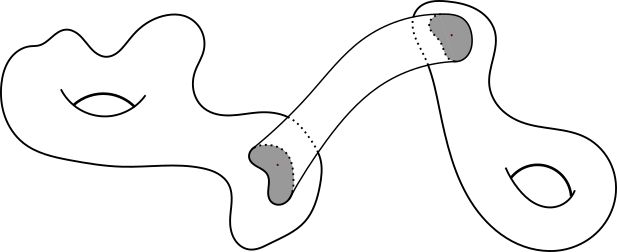
\includegraphics[width=.8\textwidth]{img/connsum.png}
    \caption{A connected sum of two manifolds. The gray areas are the embedded disks, on which the surgery is performed}\label{fig:connsum}
\end{figure}
The connection of surgeries to bordism is established in:
\begin{thesisprop}
    If $M^\prime$ is obtained from $M$ via a surgery, $[M] \equiv [M^\prime]$ in $\Omega_\ast^{\id_\BO}$.
\end{thesisprop}
\prf
Let $\iota\colon S^p \times D^q \hookrightarrow M$ be the embedding of the surgery move turning $M$ into $M^\prime$.
The so called \emph{trace} of the surgery is the space
\begin{equation*}
    W = \quotient{(M \times [0,1]) \amalg (D^{p+1}\times D^q)}{(\iota(x),1) \sim x \text{ for all } x\in S^p\times D^q \subset D^{+1}\times D^q},
\end{equation*}
which by writing it as the gluing $W = (M\times[0,1])\cup_{(\iota ,1)} (D^{p+1}\times D^q)$ is a manifold.
The boundary of this manifold is given by $M\cong M\times\{0\}$ on the one side and the surgery result $M^\prime$ on the other.
\endprf
A choice of $\t$-structures on $S^p\times D^q$ and $D^{q+1}\times S^{q-1}$ that induce the same boundary $\t$-structure on $S^p\times S^{q-1}$ allows for a well defined notion of $\t$-surgery, where one requires the embedding $\iota$ to be $\t$-preserving.
If moreover these compatible $\t$-structures on $S^p\times D^q$ and $D^{p+1}\times S^{q-1}$ are induced as the boundary $\t$-structures of a common $\t$-structure on $D^{p+1}\times D^q$, one can produce a more careful gluing of the trace, and obtain a version of the above proposition for $\t$-surgeries and $\t$-bordism.
This more careful approach can be read about in \cite{milnor:surg}, where everything is done for $\t\colon \BSO \to \BO$, but the arguments all apply to the sketched general case above.
It then turns out, that bordism and surgery are even closer related than above proposition indicates, one can for example prove statements like:
\begin{thesislemma}[thm.~1 in \cite{milnor:surg}]
    A $d$ dimensional manifold $M^\prime$ can be obtained from a $d$ dimensional manifold $M$ via a sequence of oriented surgery moves if and only if $[M] \equiv [M^\prime]$ in $\Omega_d^\BSO$.
\end{thesislemma}
Because of this lemma, we may switch the group operation in the groups $\Omega_\ast^{\BSO\to\BO}$ and $\Omega_\ast^{\id_\BO}$ away from the disjoint union $\amalg$ to the connected sum $\connsum$.
Thus, working in the unoriented bordism group, we may without loss of generality assume all representatives to be connected manifolds.
This justifies our assumption of connectedness in the rest of this thesis.


\subsection{Unoriented bordism}
The most elementary shade of bordism is unoriented bordism, that entails to picking $\t=\id\colon \BO \to \BO$ in our framework.
We call the resulting bordism ring $\NN_\ast = \Omega_\ast^{\id_\BO}$.
Since every manifold has a canonical $\id_{\BO}$-structure, we have in $\NN_d$ just all closed $d$-manifolds.
The relation is the classical bordism relation $[M] = [M^\prime]$ if and only if there exists $W$ with $\partial W \cong M \amalg M^\prime $.
The opposite of $M$ for the $\id_\BO$ structure is just $M$.
Thus every element in $\NN_\ast$ is its own additive inverse, and $\NN_\ast$ is a $\zz$-module. 
Famously, Ren\'e Thom in his thesis \cite{thom:bord} translated the question of computing the unoriented bordism groups $\NN_d$ to a question of homotopy theory, which he was then able to solve.
\begin{theorem*}[Thom, 1954]
    Two manifolds are unoriented bordant, if and only if their Stiefel--Whitney-numbers agree.
\end{theorem*}
This spectacular result marks one of the few times where the agreeing of invariants from algebraic topology gives a sufficient and not only neccesary condition for equality.
Thom moreover computed the structure of $\NN_\ast$: 
The unoriented bordism ring is a $\zz$-algebra with precicely one (multiplicative) generator in each degree $d\neq 2^k - 1$.
Furthermore, he showed that the even dimensional generators are given by the classes $[\RP^{2i}]$. 
Two years later, Albrecht Dold \cite{dold:bord} completed the picture introducing the Dold--Manifolds $P(m,n)$ we discussed \hyperlink{doldmnf}{at the end of chapter 1} and thus proving
\begin{theorem*}[Thom--Dold, 1956]
    There is an isomorphism of $\zz$-algebras
    \begin{equation*}
        \zz[x_2,x_4,x_5,x_6,x_8,x_9,\cdots]\to\NN_\ast
    \end{equation*}
    mapping $x_{i}$ to $[\RP^{i}]$ for even $i$, and $x_i$ to $[P(2^r-1,s2^r)]$ for $i = 2^r(2s + 1) - 1$ where $i$ odd and $i\neq 2^j - 1$. All numbers mentioned are nonnegative whole numbers.
\end{theorem*}
For the theorem to be well-stated we must have a unique representation of an odd number $i = 2j -1$ as a term of form $2^r(2s + 1) -1$.
This representation is of course given by the prime decomposition of the even number $2j$ giving $2j = 2^r l$ for an odd $l = 2s + 1$.
Indeed the dimensions also fit:
\begin{equation*}
    \dim \big( P(2^r -1 , s2^r) \big) = \dim \big( S^{2^r -1} \times \CP^{s2^r} /_\sim \big) = (2^r - 1) + (2(s2^r)) = 2^r(2s + 1) - 1 = i.
\end{equation*}
Thus we may interpret the index of the generators as the degree and obtain an isorphism of graded algebras. 
In the following text, we will use the symbol $x_i$ interchangable with its image under this isomorphism.\\
The additive structure of $\NN_\ast$ will be of more importance than the multiplicative structure for this work, so we shift our attention there.
How many additive generators are there in dimension $d$?
Since every additive generator is built from a collection of multiplicative generators with totaled dimension $d$, we have a one--to--one-correspondence
\begin{equation*}
    \begin{Bmatrix} \text{Partitions } (i_1, \dots ,i_k) \\ \text{ of } d = i_1 + \dots + i_k \\ \text{ with } i_\ast \neq 2^j - 1 \end{Bmatrix} \overset{1:1}{\longleftrightarrow}
    \begin{Bmatrix} \text{Additive generators } \\ x_{i_1} \cdots x_{i_k} \text{ of } \NN_d \end{Bmatrix}
\end{equation*}
So the dimension of $\NN_d$ as a $\zz$-vectorspace is given by the amount $a(d)$ of such partitions of $d$ that dont allow Mersenne-numbers, \ie elements of the form $2^j - 1$.
As bordism classes are simply elements of the vector space $\NN_d$, the amount of bordism classes of manifolds of dimension $d$ is hence given by $2^{a(n)}$.
\begin{figure}
    \centering
    \includegraphics[width=\textwidth]{img/tikz/ubord.pdf}
    \caption{The dimensions $a(d)$ of $\NN_d$ as a $\zz$-module, \href{https://oeis.org/A078657}{Sequence A078657} in the online Encyclopedia of integer sequences. Also contains the amount $2^{a(d)}$ of distinct bordism classes in $\NN_d$.}\label{fig:ubord}
\end{figure}
See \fref{fig:ubord} for some lowdimensional examples.
Just by these few observations we have casually shown that every closed $3$-manifold arises as the boundary of a $4$-manifold, demonstrating the power of these results.\\
To shed more light on Thom's first theorem, recall that the Stiefel--Whitney-number of a $d$-Manifold $M$ corresponding to the partition $(i_1,\dots , i_k)$ of $d= i_1 + \dots + i_k$ is given by 
\begin{equation*}
    \langle w_{i_1}(M) \smile \cdots \smile w_{i_k}(M) , [M]\rangle
\in \zz
\end{equation*}
where $[M]$ denotes the $\zz$-fundamental class of $M$.
We will now as an example compute the Stiefel--Whitney-numbers of some manifolds to illustrate the process.
As we have already seen, the total Stiefel--Whitney-class of $\CP^2$ is given by $(1 + b)^3$ with $\deg(d) = 2$, so we obtain \begin{equation*}
    w_1 = 0, w_2 = b, w_3 = 0, w_4 = b^2
\end{equation*}
There are five partitions of $d = 4$, giving rise to the top degree $H^4(\CP^2;\zz)$ classes 
\begin{equation*}
    \begin{split}
        w_1\smile w_1 \smile w_1 \smile w_1 & \leftrightarrow 0 \\
        w_1\smile w_1 \smile w_2 & \leftrightarrow 0 \\
        w_1\smile w_3 & \leftrightarrow 0 \\
        w_2\smile w_2  & \leftrightarrow b^2 \\
        w_4  & \leftrightarrow b^2 
    \end{split}
\end{equation*}
By Poincar\'e-duality, the fundamental class $[\CP^2]$ is the dual of the unique nontrivial element $b^2 \in H^4(\CP^2;\zz)$.
Therefore pairing above classes with the fundamental class simply amounts to counting occurences of $b^2$ modulo two.
We therefore get only two nonzero Stiefel--Whitney-numbers, the one corresponding to $(2,2)$ as well as the one corresponding to $(4)$.\\
As a second example, let us compute the Stiefel--Whitney-numbers of $\RP^2\times \RP^2$, another nontrivial element in $\NN_4$.
The total Stiefel--Whitney-class is given by the Whitney product theorem as $w = (1 + a)^3(1 + b)^3$ with relations $a^3 = b^3 = 0$.
We thus obtain the Stiefel--Whitney-classes
\begin{equation*}
    w_1 = a + b, w_2 = a^2 + ab + b^2, w_3 = a^2 b + a b^2, w_4 = a^2 b^2
\end{equation*}
Computing for each partition the product of those classes yields
\begin{equation*}
    \begin{split}
        w_1\smile w_1 \smile w_1 \smile w_1 & \leftrightarrow a^4 + b^4 = 0 \\
        w_1\smile w_1 \smile w_2 & \leftrightarrow (a^2 + b^2)(a^2 + ab + b^2) = 0 \\
        w_1\smile w_3 & \leftrightarrow (a + b)(a^2 b + b^2 a) = 2a^2 b^2 = 0 \\
        w_2\smile w_2  & \leftrightarrow 3 a^2b^2 = a^2b^2\\
        w_4  & \leftrightarrow a^2b^2 
    \end{split}
\end{equation*}
Then after counting the occurences of the top class $a^2b^2$, we have again only the same two nonvanishing Stiefel--Whitney-numbers as with $\CP^2$.
Applying the theorem of Thom, we have shown that $\CP^2$ and $\RP^2 \times \RP^2$ are bordant.
This is by no means a coincidence, as first noted (hearsay, as it is in russian) by Vladimir Rokhlin in \cite{rokhlin:bord}:
\begin{thesislemma}[Rokhlin's trick]\label{rokhlintrick}
    For all $n$ the $2n$-manifolds $\RP^n \times \RP^n$ and $\CP^n$ are bordant.
\end{thesislemma}
\prf
This proof is just a slightly expanded version of the original proof of Wall in \cite{wall:bord}.
By the theorem of Thom, it suffices to give an argument why all Stiefel--Whitney-numbers of the manifolds agree.
First note, that for any manifold $M$ we have by the Whitney product theorem and the symmetry of the cup product
\begin{equation*}
    w_k(M\times M) = \sum\limits_{i + j = k} w_i(M)\smile w_j(M) = 
    \begin{cases} 0 & k \text{ odd,} \\ w_{k/2}(M) \smile w_{k/2}(M) & k \text{ even.} \end{cases}
\end{equation*}
Thus any Stiefel--Whitney-number containing an odd element in the partition automatically vanishes.
Moreover, for any strictly even partition $(2i_1,\dots ,2i_k)$ we calculate
\begin{equation*}
    w_{2i_1}(M\times M)\smile \cdots \smile w_{2i_k}(M\times M)
    = \big(w_{i_1}(M) \smile \cdots \smile w_{i_k}(M)\big)^{\smile 2} 
\end{equation*}
Pairing this with the fundamental class $[M\times M] = [M]\otimes [M]$ using the Künneth-theorem, we get the square of the Stiefel--Whitney-number of $M$ corresponding to $(i_1,\dots ,i_k)$.
In $\zz$, an element is zero if and only if its square is zero.
Thus nonzero Stiefel--Whitney-numbers of $M$ are in one to one correspondence with those of $M\times M$ by "doubling" partitions.\\
The total Stiefel--Whitney-class $(1 + b)^{n+1}$ of $\CP^n$ may be obtained from the total Stiefel--Whitney-class $(1+a)^{n+1}$ of $\RP^n$ by formally doubling the degree of the generator $a$.
Therefore the Stiefel--Whitney-classes of $\CP^n$ are also obtained from those of $\RP^n$ by formally doubling degrees, and equally the Stiefel--Whitney-numbers by doubling partitions.
Hence the Stiefel--Whitney-numbers of $\CP^n$ and $\RP^n\times\RP^n$ agree.
\endprf
We note that exactly the same proof shows $[\CP^n\times\CP^n] = [\HP^n]$ since again $w(\HP^n) = (1 + c)^{n+1}$ for a sole degree $4$ generator $c$ of $H^\ast(\HP^n;\zz)$ subject only to the relation $c^{n+1}=0$.
The above proof is as simple as it is unsatisfying,
Wall indeed comments:
\say{The author feels that it ought to be proved by constructing a manifold with appropriate boundary, but has been unable to find one}.
In a cute and very explicit two-page paper \cite{stong:cob}, Stong provides such a manifold twelve years later.
Combining the above with our knowledge of the ring $\NN_\ast$, we obtain the more general
\begin{thesisprop}
    The square $M\times M$ of any manifold $M$ is bordant to an orientable manifold.
\end{thesisprop}
\prf
Write $M$ as a product of generators $x_i$.
The square of a product is the product of the squares.
If $i$ is even, the above lemma gives $x_i^2 = [\CP^n]$ which is orientable. 
If $i$ is odd, the Dold-manifold $x_i = [P(2^r - 1, s2^r)]$ has odd first entry and even second entry.
Thus by our computation in \fref{fig:pmn}, the Dold-manifold is already orientable and so is its square.
\endprf
Again a more direct construction of such a bordism would be desirable, Wall notes.
As to our knowledge, no such construction exists to the present day. 
There is another view on this proposition:
On an orientable manifold, every Stiefel--Whitney-number containing a copy of $w_1$ vanishes.
A neccesary condition for a manifold to be bordant to something orientable thus by Thom's theorem given by the vanishing of all Stiefel--Whitney-numbers containing a $1$ in the partition.
It is not too hard to prove, that this condition is actually also sufficient, we refer to \cite{wall:bord} but skip the proof here as it neccesitates some discussion of the oriented bordism ring.
As we have computed, on any square $M\times M$ all odd Stiefel--Whitney-classes vanish, giving another proof of the proposition since $1$ is an odd number.
Since we saw that the odd Stiefel--Whitney-classes all vanish on any square, in the same spirit one could ask
\begin{q}
    Let $M$ be a even dimensional manifold such that all Stiefel--Whitney-numbers of $M$, that contain an odd number in their corresponding partition vanish.
    Is $M$ bordant to a square $N\times N$?
\end{q}\noindent{}
The answer to this question eludes us for now.
We will instead continue using our gained knowledge to describe a general additive generator of the bordism ring $\NN_\ast$.
\begin{thesisprop}\label{eprop}
    Call $\mathcal{E}$ the set containing all manifolds of form
    \begin{equation*}
        \prod\limits_{i\in I} (\CP^i)^{n_i} \times \prod\limits_{j\in J} (\RP^{2j})^{o_j} \times \prod\limits_{k\in K}{P(2^{r_k} - 1,s_k2^{r_k})}
    \end{equation*}
    with $I,J,K$ finite subsets of the natural numbers, $n_i,r_k,s_k$ positive natural numbers and $o_j \in \{0,1\}$.
    Then $\mathcal{E}$ generates $\NN_\ast$ additively.
\end{thesisprop}
\prf
As discussed, the set of products of form $\prod_{j\in J} x_j^{n_j}$ is a set of additive generators.
Factoring out the even powers of even $x_i$ and applying \hyperref[rokhlintrick]{Rokhlin's trick} repeatedly gives the result.
\endprf
We conclude this chapter with a verbose list of the additive generators of $\NN_\ast$ in the first couple dimensions following the notation of the proposition, see \fref{fig:boboring}
\begin{figure}
    \centering
    \includegraphics[width=\textwidth]{img/tikz/boboring.pdf}
    \caption{Additive generators of the first fourteen unoriented bordism groups.}\label{fig:boboring}
\end{figure}
This list, as well as the highly algorithmic computations of Stiefel--Whitney-numbers in this chapter have of course been generated or verified with computer assistance.
For a neat Haskell-program performing these sorts of computations, see \hyperlink{appendix}{the appendix of this work}.

\clearpage

% Chapter 3
\section{Positive scalar curvature}\label{sec:psc}
As the spirit of this work is demonstrating how to prove theorems about positive scalar curvature with minimal knowledge of positive scalar curvature, we begin the first part of this chapter by only a very brief and by no means exhaustive introduction to scalar curvature, following \cite{stolz:survey} and \cite{carl:survey}.
Subsequently, we give an overview of the results from our basis \cite{ew:psc} that are needed in our proof.\\
In the \hyperlink{subsection.3.2}{second part of this chapter}, we then state and prove our main theorem.
Exactly like promised in the introduction, the proof will proceed by using the results from the first part to show that most of the additive generators $\mathcal{E}$ from \ref{eprop} admit an admissible splitting.
\subsection{Preliminaries}
We choose the most geometrical definition of the three main approaches mentioned in \cite{carl:survey}.
\begin{defi}[Scalar curvature]
Let $(M,g)$ be a riemannian manifold of dimension $n$. 
The scalar curvature of $g$ is the function $\scal_g\colon M\to \R$ that appears in the third coefficient
\begin{equation*}
    \frac{\vol(B_r(x))}{\vol(B_r^{\text{euklid}})} = 1 - \frac{\scal_g(x)}{6(n+2)}r^2 + \dots
\end{equation*}
    of the taylor expansion comparing the metric volume of a radius $r$ metric ball $B_r(x)\subset M$ around $x$ with the usual euclidian volume of the ball $B_r^{\text{euclid}} = \{x \in \R^n \:\vert\: \lVert x \rVert \leq r\}$.
\end{defi}
We instantly obtain that the scalar curvature of euclidean space $\R^n$ with the usual flat euclidean metric is zero.
Furtheremore, if $(M,g)$ is a riemannian manifold, and $G$ is a discrete group acting freely on $M$ by isometries, then we obtain an induced metric $g^\prime$ on the quotient $M^\prime = M/_G$.
With this metric, the canonical projection $p\colon M\to M^\prime$ is a local isometry, and we hence have $\scal_g(x) = \scal_{g^\prime}(p(x))$.
Thus the Torus $T^n = \R^n/\Z^n$ also has a flat metric of scalar curvature zero.
\begin{defi}[\psc]
    A metric $g$ on a manifold $M$ is called \psc-metric, if $\scal_g > 0$ everywhere. A manifold $M$ is called \psc-manifold, if it admits such a metric
\end{defi}
The unit sphere $S^n\subset \R^{n+1}$ is the primary example of a \psc-manifold.
We denote its metric by $g_{\text{round}}$.
As can be easily calculated, its scalar curvature is constant, and given by 
\begin{equation*}
    \scal_{g_{\text{round}}}(x) = n(n-1)
\end{equation*}
By the same argument as above, $\RP^n = S^n/_{\zz}$ is thererfore also a \psc-manifold.
The following are direct consequences of the definition and some calculation:
\begin{thesislemma}
    Let $(M,g)$ and $(M^\prime, g^\prime)$ be riemannian manifolds and $\lambda\in\R^+$. Then
    \begin{enumerate}[label=\roman*.,noitemsep]
        \item $\scal_{g\oplus g^\prime}(x,x^\prime) = \scal_g(x) + \scal_{g^\prime}(x^\prime)$ for any $(x,x^\prime)\in M\times M^\prime$.
        \item $\scal_{\lambda g}(x) = \frac{1}{\lambda} \scal_g(x)$ for all $x\in M$.
    \end{enumerate}
\end{thesislemma}
Gromov even advocates an axiomatic characterization of scalar curvature \cite{grom:four}, consisting of the two properties from the lemma as well as a normalization and a volume comparison property.
Thus the two properties from the lemma ought to be the only thing we need when proving simple statements about scalar curvature, such as this first existence result.
\begin{thesisprop}\label{prodpsc}
    Let $g$ be a \psc-metric on $M$, and $M^\prime$ any manifold. Then $M\times M^\prime$ admits a \psc-metric.
\end{thesisprop}
\prf
Choose any metric $g^\prime$ on $M^\prime$.
By compactness, $\scal_{g^\prime} \geq -k$ for some $k\in \N$.
Similarly by compactness, there exists an $\varepsilon > 0$ with $\scal_g \geq \varepsilon$.
Consider the metric $tg \times g^\prime$ on $M\times M^\prime$ with $t < \varepsilon / k$.
By above lemma we compute
\begin{equation*}
    \scal_{tg \times g^\prime}(x,x^\prime) = \frac{1}{t}\scal_g(x) + \scal_{g^\prime}(x^\prime) > \frac{k}{\varepsilon} \varepsilon - k = 0.
\end{equation*}
Hence we have found a metric of positive scalar curvature.
\endprf
Intuitively, the above proof is described by shrinking $M$ to blow up the scalar curvature.
A way more difficult existence result, the proof of which goes way beyond the scope of this exposition, is the famous surgery result from \cite{gl:scpsc} and \cite{sy:scpsc}.
\begin{theorem*}[Gromov--Lawson--Schoen--Yau, 1979-1980]
    Let $M$ be a \psc-manifold and $M^\prime$ be any manifold which can be obtained from $M$ by a codimension $3$ surgery. Then $M^\prime$ admits a \psc-metric too.
\end{theorem*}
As an immediate application, the connected sum $M\connsum M^\prime$ (a dimension $0$ surgery) of two $n$-dimensional \psc-manifolds $M,M^\prime$ admits a \psc-metric if $n\geq 3$.
This theorem was the begin of the connection of scalar curvature to bordism that ultimately results in a variant of Chernysh's theorem proven in this generality first in \cite{georg:diss}.
\begin{theorem*}[Chernysh, 2004]
    Let $M,M^\prime$ be two $d$-dimesional manifolds of tangential $2$-type $\t$. 
    Then $[M]\equiv [M^\prime]$ in $\Omega_d^\t$ implies $\mR^+(M) \whe \mR^+(M^\prime)$.
\end{theorem*}
It shows how to compare the spaces of \psc-metrics for bordant manifolds. 
Such a comparison theorem for nonbordant manifolds is the 
theorem which we wish to apply to obtain our result:
\begin{theorem*}[Ebert--Wiemeler, 2022]
    Let $M$ and $M^\prime$ be $d$-Manifolds of tangential $2$-type $(B,\t)$ and $x\in \Omega_d^\t$ a bordism class containing a representative with \emph{admissible splitting}, such that $[M] \equiv [M^\prime] + x$ in the $\t$-bordism group $\Omega_d^\t$, then there is a weak homotopy equivalence
    \begin{equation*}
        \mR^+(M) \whe \mR^+(M^\prime)
    \end{equation*}
    provided that $d\geq 5$.
\end{theorem*}
To syntactically understand the above theorem we need to introduce the space of metrics, explain its topology, and introduce the notion of admissible splittings.
Let us begin with the former:
A riemannian metric on $M$ is but a smooth choice of nondegenerate bilinear mappings $T_pM\times T_p M\to \R$ for each $p\in M$, or in other words a smooth section of the bundle $T^\ast M \otimes T^\ast M \to M$.
The space of all such sections $\Gamma (T^\ast M \otimes T^\ast M)$ may be given the usual $C^\infty$-topology, since $M$ is compact.
We than equip
\begin{equation*}
    \mR^+(M) = \{ g \:\vert\: g \text{ riemannian metric with } \scal_g > 0\} \subset \Gamma(T^\ast M \otimes T^\ast M )
\end{equation*}
with the subspace topology.
We move on towards the definition of an admissible splitting.
Let $W$ be a $\t$-bordism $M_0\bord M_1$, and $h_0,h_1$ riemannian metrics on $M_0,M_1$. 
We denote 
\begin{equation*}
    \mR^+(W)_{h_0,h_1} = \{ g \text{ riem.~ metric on } W \:\vert\: g = h_i\oplus dt^2 \text{ around } M_i, \scal_g >0\}.
\end{equation*}
It is the space of \psc-metrics on $W$ that are locally of product form at the boundary and restrict to the given metrics $h_i$ there.
By additivity, $\scal_g > 0$ implies $\scal_{h_i} > 0$, so $\mR^+(W)_{h_0,h_1} = \emptyset$ whenever one of the $h_i$ is not \psc.
Given another bordism $W^\prime\colon M_1 \bord M_2$, there is a gluing map 
\begin{equation*}
    \mu_{W,W^\prime}\colon \mR^+(W)_{h_0,h_1} \times \mR^+(W^\prime)_{h_1,h_2} \to \mR^+(W\cup_{M_1} W^\prime)_{h_0,h_2}
\end{equation*}
which sends $(g,g^\prime)$ to $g\cup g^\prime$, which is well defined as $g$ and $g^\prime$ are locally of product form around $M_1$ and hence agree at $M_1$.
We call a metric $g\in\mR^+(W)_{h_0,h_1}$ on $W\colon M_0\bord M_1$ right stable, if for all riemannian manifolds $(M_2,h_2)$ with $\scal_{h_2}>0$ and all $W^\prime\colon M_1 \bord M_2$ the partial gluing map
\begin{equation*}
    \mu_{W,W^\prime}(g,\bullet)\colon \mR^+(W^\prime)_{h_1,h_2} \to \mR^+(W\cup_{M_1} W^\prime)_{h_0,h_2}
\end{equation*}
is a weak homotopy equivalence.
Call the metric $g$ in strong analogy left stable, if for all riemannian manifolds $(M_{-1},h_{-1})$ with $\scal_{h_{-1}}>0$ and all bordisms $W_\prime\colon M_{-1}\bord M_0$ the partial gluing map $\mu_{W_\prime,W}(\bullet,g)$ is a weak equivalence.
\begin{defi}[Admissible splitting]
    An admissible splitting of a (closed) $d$-manifold is a decomposition $M = M_0\cup_{N} M_1$ into two bordisms
    \begin{equation*}
        \emptyset \overset{M_0}{\bord} N \overset{M_1}{\bord} \emptyset
    \end{equation*}
    such that the inclusions $N\hookrightarrow M_i$ are $2$-connected and there are metrics $h_i\in\mR^+(N)$ and $g_i \in \mR^+(M_i)_{h_i}$ such that ...
    \begin{enumerate}[noitemsep, label=...]
        \item $g_0$ is right stable
        \item $g_1$ is left stable
        \item $h_0$ and $h_1$ are in the same path-component of $\mR^+(N)$.
    \end{enumerate}
\end{defi}
Any manifold admitting an admissible splitting is a \psc-manifold.
Take any path $h_t$ from $h_0$ to $h_1$ and interpret it as a \psc-metric $h_\bullet\in\mR^+(N\times[0,1])_{h_0,h_1}$. 
Then by gluing we obtain a \psc-metric $g_0\cup h_\bullet \cup g_1$ on $M_0\cup_N N\times[0,1]\cup_N M_1$.
The latter is diffeomorphic to $M$ so $M$ admits a \psc-metric.\\
Ebert and Wiemeler give a result to construct manifolds with admissible splittings from manifolds with a decomposition into disk bundles, which will be key to our proof in the next section.
It is to be viewed as an analogue of \ref{prodpsc} for admissible splittings.
\begin{thesislemma}[Ebert--Wiemeler, prop.~5.2 in \cite{ew:psc}]\label{diskbdlsplit}
    Let $E_i \to M_i$ be two rank $n\geq 3$ vector bundles. 
    Let $M$ be obtained by gluing together their disk bundles $M = D(E_1)\cup_\psi (-D(E_2))$ along a diffeomorphism $\psi\colon S(E_1) \to S(E_2)$. 
    Let $M^\prime$ be any manifold that admits a \psc-metric. Then $M\times M^\prime$ has an admissible splitting.
\end{thesislemma}
Taking this lemma into consideration led to a significantly streamlined version of the proof of our main theorem below.
Our thanks go to Johannes Ebert for reminding the author via email of its importance, which was originally overlooked.


\subsection{The main result}
We specialize to the case $\t= \id\colon \BO \to \BO$. 
Every manifold is then a canonically a $\t$-manifold.
By our classification result \ref{tttypes}, a manifold $M$ has tangential $2$-type $\id_\BO$, which is in the first type family, if and only if it satisfies
\begin{enumerate}[label=(\alph*), noitemsep]
    \item The manifold has fundamental group $\pi_1(M) \cong \zz$.
    \item The manifold is nonorientable by $w_1(M)\neq 0$.
    \item The universal cover of $M$ is nonspinnable by $w_2(\widetilde{M}) \neq 0$.
\end{enumerate}
Let us fix a dimension $d$.
Suppose that $\mathcal{E}_d$ is some set generating additively the unoriented bordism group $\NN_d$.
Define
\begin{equation*}
    \mathcal{E}_d^{\text{good}} = \{ x \in \mathcal{E}_d \:\vert\: x \text{ contains a representative with admissible splitting}\}
\end{equation*}
And call $\mathcal{A}_d$ the subgroup of $\NN_d$ generated by $\mathcal{E}_d^\text{good}$.
Then we may apply the theorem from \cite{ew:psc} to obtain the following 
\begin{blueprint*}
    \color{themecolordark}
    Two $d$-dimensional manifolds $M,M^\prime$ satisfying (a),(b),(c) with $[M] \equiv [M^\prime]$ in $\NN_d / \mathcal{A}_d$ have
    \begin{equation*}
        \mR^+(M) \whe \mR^+(M^\prime)
    \end{equation*}
    provided that $d\geq 5$.
\end{blueprint*}
\prf
Notice that the elements in $\NN_d$ which contain a representative with an admissible splitting form a subgroup, since admissible splittings may be constructed componentwise in a disjoint union.
Thus $[M] \equiv [M^\prime]$ in $\NN_d / \mathcal{A}_d$ implies there is a $x\in\NN_d$ with a representative which admits an admissible splitting and $[M] = [M^\prime] + x$.
Then the theorem of Ebert--Wiemeler applies.
\endprf
All there is left to to, is to find as many manifolds with admissible splitting in our list $\mathcal{E}$ from \ref{eprop} as possible.
Thankfully, Ebert and Wiemeler provide a multitude of such manifolds in section 3 of their paper.
We will first use the following result of theirs to show that most of our generators have an admissible splitting.
Shortly after, we will then spruce up the result with \ref{diskbdlsplit}, to obtain even more admissible splittings.
\begin{thesislemma}[Ebert--Wiemeler, thm 3.1 in \cite{ew:psc}]
    Let $M \to M^\prime$ be a smooth fiber bundle with fiber $\KP^{n + m - 1}$. Then $M$ has an admissible splitting if either ...
    \begin{enumerate}[label=$\dots$, noitemsep]
        \item $\K = \R$, $n,m\geq 3$ and the bundle has structure group $O(m)\times O(n) / \{\pm 1\}$
        \item $\K = \C$, $n,m \geq 2$ and the bundle has structure group $U(n)\times U(m)$.
        \item $\K = \C$, $n + m -1 \geq 3$ with structure group $\zz$ acting by complex conjugation.
        \item $\K = \HH$, $n,m\geq 1$ and the bundle has structure group $\mathrm{Sp}(n)\times\mathrm{Sp(m)}/\{\pm 1\}$
    \end{enumerate}
\end{thesislemma}
As a direct corollary, any product $\RP^d\times M^\prime$ with $d \geq 5$ has an admissible splitting, as a trivial bundle admits a structure group reduction to the trivial group, and thus fulfills any such requirement.
By the same argument, any product $\CP^d\times M^\prime$ with $d\geq 3$ also admits admissible splitting, and any product $\HP^d \times M^\prime$ with $d\geq 1$ similarly. 
Furthermore, the Dold-manifold $P(m,n)$ is the total space of smooth a fiber bundle 
\begin{equation*}
    \CP^n \fib P(m,n) \overset{p}{\longrightarrow} \RP^m
\end{equation*}
with $p([x,z]) = [x]$. 
The transition maps perform complex conjugation, so the structure group of this fiber bundle is $\zz$, see \cite{dold:bord}.
For $n\geq 3$ therefore also $P(m,n)$ has an admissible splitting, and any product $P(m,n)\times M^\prime$ hence too.
To summarize,
any element in $\mathcal{E}$ with a representative accomodationg a factor of a suitably high dimensional projective space or Dold-manifold will have an admissible splitting.
This already includes most elements. In fact:
\begin{thesisprop}\label{fbo}
    All elements in $\mathcal{E}$ contain a representative with admissible splitting, except maybe those represented by a manifold of form
    \begin{equation*}
        (\CP^2)^{o_4} \times (\RP^2)^{o_1} \times (\RP^4)^{o_2} \times P(1,2)^k
    \end{equation*}
    with $o_i \in \{0,1\}$ and $k\in \N_0$.
\end{thesisprop}
\prf
By \ref{eprop} a general element in $\mathcal{E}$ is represented by 
\begin{equation*}
    M = \prod\limits_{i\in I} (\CP^{2i})^{n_i} \times \prod\limits_{j\in J} (\RP^{2j})^{o_j} \times \prod\limits_{k\in K}{P(2^{r_k} - 1,s_k2^{r_k})}
\end{equation*}
    with $I,J,K$ finite subsets of the natural numbers, $n_i,r_k,s_k$ positive natural numbers and $o_j \in \{0,1\}$.
    If $n_i$ is nonzero for some $i\geq 2$, we have a factor of $\CP^d$ with $d\geq 4$, so $M$ has an admissible splitting.
    If $o_j$ is nonzero for some $i\geq 3$, we have a factor of $\RP^d$ with $d\geq 6$, so $M$ has an admissible splitting.
    Since $s_k 2^{r_k} < 3$ only for $s_j = r_j = 1$, the only Dold-manifold whose appearance does not a priori make the product have an admissible splitting is $P(1,2)$.
    We are thus left with manifolds of form
\begin{equation*}
    M = (\CP^2)^{n_1} \times (\RP^2)^{o_1} \times (\RP^4)^{o_2} \times P(1,2)^{n_2}
\end{equation*}
    with $n_i\in \N_0$ and $o_i\in\{0,1\}$.
    Using Rokhlin's-trick, if $n_1\geq 2$ we obtain a factor $\HP^2$ from $\CP^2\times\CP^2$, and the product again has an admissible splitting.
    Thus it suffices to consider $n_1\in \{0,1\}$.
\endprf
%Since $P(1,2)$ is fivedimensional, $P(1,2)^k$ has dimension $5k> 6$ if $k \geq 2$.
%Furthermore $P(1,2)$ is orientable, hence by \ref{prodlem} any product $P(1,2)^2 \times M^\prime$ with nontrivial $M^\prime$ is bordant to a manifold with an admissible splitting.
%We may thus reduce the list of outliers further.
%\begin{thesisprop}[Refinement of \ref{fbo}]\label{plo}
    %All elements in $\mathcal{E}$ contain a representative with admissible splitting, except maybe those represented by 
    %\begin{equation*}
        %\begin{split}
        %\RP^2, \CP^2, \RP^4, \RP^4\times\RP^2, \CP^2\times\RP^2, \CP^2\times\RP^4, \CP^2\times\RP^4\times\RP^2, P(1,2),  \\
           %P(1,2)^2, P(1,2)\times\RP^2, P(1,2)\times \CP^2, P(1,2)\times\RP^4, P(1,2)\times\RP^4\times\RP^2
        %\end{split}
    %\end{equation*}
    %In particular all elements of dimension $d>11$ contain a representative with admissible splitting.
%\end{thesisprop}
%\prf
%As both $P(1,2)\times P(1,2)$ and $P(1,2)\times\CP^2$ are orientable manifolds of dimension larger then six, \ref{prodlem} applies to any product of form $P(1,2)^2\times M^\prime$ and $P(1,2)\times \CP^2 \times M^\prime$ with nontrivial $M^\prime$.
%This refines \ref{fbo} to the given list.
%\endprf
%This leaves only finitely many outliers, which is a marvellous start, but further refinement remains possible.
Let us refine the result further.
Not only do Ebert and Wiemeler prove that $[P(1,2)]$ has a representative with an admissible splitting, they give an explicit construction of a certain $5$-manifold which satisfies:
\begin{thesislemma}[Ebert--Wiemeler, prop.~5.8 in \cite{ew:psc}]\label{pundoes}
    There is a five manifold $W$ which has an admissible splitting $W=W_0 \cup W_1$ with $W_i$ two $D^3$-bundles over $S^2$ such that $[W]\neq 0$ in the oriented bordism group $\Omega_5^{\BSO\to\BO}$.
\end{thesislemma}
Already Wall computed in \cite{wall:bord} that $\Omega_5^{\BSO\to\BO}  = \zz$ and the orientation forgetting map from $\Omega_5^{\BSO\to\BO}$ to $\NN_5$ is an isomorphism.
Hence the manifold $W$ from the theorem satisfies $[W] \equiv [P(1,2)]$ in $\NN_5$.
Of course this disk bundle decomposition is precicely what is needed for an application of \ref{diskbdlsplit}.
Taking the representative $W\times M^\prime$ for products of form $[P(1,2)\times M^\prime]$, we have an representative that has an admissible splitting, when $M^\prime$ has a \psc-metric.
Iterated application results in:
\begin{thesisprop}[Refinement of \ref{fbo}]
    All elements in $\mathcal{E}$ contain a representative with admissible splitting, except maybe those represented by 
    \begin{equation*}
        \RP^2, \CP^2, \RP^4, \RP^4\times\RP^2, \CP^2\times\RP^2, \CP^2\times\RP^4, \CP^2\times\RP^4\times\RP^2.
    \end{equation*}
    In particular all elements of dimension $d>10$ contain a representative with admissible splitting.
\end{thesisprop}
\prf
The Dold-manifold $P(1,2)$ has a representative $W$ with admissible splitting by \ref{pundoes}, so it drops from the list of outliers in \ref{fbo}.
This representative also admits a \psc-metric by our remark after the definition of admissible splittings,
so we may apply \ref{diskbdlsplit} also to pure products $P(1,2)^k$, removing them from the list.
By \ref{prodpsc} any product $\RP^k\times M^\prime$ admits a \psc-metric, so \ref{diskbdlsplit} applies to products $P(1,2)\times\RP^k\times M^\prime$ , and those drop from the list in \ref{fbo}.
By representing $\CP^2$ as $\RP^2\times\RP^2$ with the same argument $[P(1,2)\times\CP^2\times M^\prime]$ has a represenative with an admissible splitting (it can of course also be shown more directly that $\CP^2$ admits a \psc-metric, leading to the same result).
We hence have removed all occurences of $P(1,2)$ from the list of outliers, giving the desired result.
\endprf
There is an alternative proof that $P(1,2)$ admits a \psc-metric utilizing a theorem from Gromov--Lawson:
The fibration $\CP^2 \fib P(1,2) \to S^1 = \RP^1$ gives the LES
\begin{equation*}
    0 = \pi_1(\CP^2) \to \pi_1(P(1,2)) \overset{p_\ast}{\longrightarrow} \pi_1(S^1) \to \pi_0(\CP^2) = 0
\end{equation*}
So we get a generator $p_\ast^{-1}(\id_S^1) \in \pi_1(P(1,2)) \cong \Z$.
This generator is represented by an embedding $S^1\to P(1,2)$ as $2\dim(S^1) + 1 = 3 < 5 = \dim(P(1,2))$. 
Since $P(1,2)$ is orientable, this embedding has trivial normal bundle, so we may thicken it to an embedding $S^1\times D^{4} \to P(1,2)$.
Performing a dimension $2$ surgery move we replace this $S^1\times D^{4}$ by a $D^2 \times S^3$, killing the generator of $\pi_1(P(1,2))$ in the process.
We obtain a simply connected five dimensional manifold, which by \cite{gl:scpsc} admits a \psc-metric.
As $5-2 = 3 \geq 3$, the codimension of the surgery was big enough, so that we may conclude $P(1,2)$ admits a \psc-metric aswell.
This killing of $\pi_1$ marks just one incidence of a general result obtainable with surgery theory. 
Any manifold whose tangent bundle trivializes over the $k$-skeleton can be made $k$-connected with surgery moves, see \cite{milnor:surg}.\\
Let us continue towars the main theorems.
In the notation of the {\color{themecolordark} blueprint} the proposition translates to $\mathcal{E}_d^{\text{good}} = \mathcal{E}_d\setminus \mathcal{E}_d^{\text{bad}}$ where 
\begin{equation*}
    \begin{split}
        \mathcal{E}_6^\text{bad} &= \{\CP^2\times\RP^2, \RP^4\times\RP^2\}\\
        \mathcal{E}_8^\text{bad} &= \{\CP^2\times\RP^4\}\\
        \mathcal{E}_{10}^\text{bad} &= \{\CP^2\times\RP^4\times \RP^2\}
    \end{split}
\end{equation*}
and empty $\mathcal{E}_d^\text{bad}$ for $d\geq 5$ else. 
We omit of course the dimesions $1,2,3,4$ where our theorems have no grip.
With a swift look at \fref{fig:boboring} containing our table of the additive generators of the lowdimensional groups $\NN_d$, we compute the quotient $\NN_d/\mathcal{A}_d$ to be $\{S^d\}$ for $d$ odd or $d>10$, and 
\begin{equation*}
    \begin{split}
        \NN_2/\mathcal{A}_6 &= \{S^6, \CP^2\times\RP^2, \RP^4\times\RP^2, (\CP^2\times\RP^2) \connsum (\RP^4\times\RP^2)\}\\
        \NN_2/\mathcal{A}_8 &= \{S^8, \CP^2\times\RP^4\}\\
        \NN_2/\mathcal{A}_{10} &= \{S^{10}, \CP^2\times\RP^4\times\RP^2\}
    \end{split}
\end{equation*}
At last, we use our {\color{themecolordark} blueprint}. 
We obtain three almost identical theorems for the exceptional dimensions $d=6,8,10$, and one general theorem for all other dimensions $d\geq 5$.
In dimension $1,2$ and $3$, the universal cover of any manifold is trivially spinnable as discussed, so there are no manifolds of tangential $2$-type $\id_\BO$ in these dimensions. 
Hence vacuously any (nonexistant) such manifold of odd dimension $d< 5$ satisfies whatever we may wish.
Applying our {\color{themecolordark} blueprint} to all the cases where $\NN_d/\mathcal{A}_d$ is the trivial group yields:
\begin{theorem}[Large or odd dimensions]
    Let $d\in \N$ be odd or $d>10$. Let $M,M^\prime$ be any two $d$-dimensional manifolds of tangential $2$-type $\id_\BO$. Then $\mR^+(M) \whe \mR^+(M^\prime)$.
\end{theorem}
For even $d\geq 6$ we know Dold--manifolds of tangential $2$-type $\id_\BO$, namely write $d= 4k + 3 + (-1)^k$ for a unique $k\in\N$, then $P(3 + (-1)^k,2k)$ is a Dold-manifold of type $\id_\BO$ in dimension $d$ by our table in \fref{fig:pmn}. 
Alternatively, manifolds of form $S^{d-6}\times\CP^2\times\RP^2$ of course give examples of nullbordant manifolds satisfying (a),(b),(c) in dimensions $d\geq 8$ or $d=6$.
We write our theorem more concretely using these manifolds and the transitivity of $\whe$:
\begin{theorem}[Explicit version of theorem 1]
    Let $d\in\N$ satisfy $d=9$ or $d> 10$, and $M$ be a $d$-dimensional manifold of tangential $2$-type $\id_\BO$. Then
    \begin{equation*}
        \mR^+(M) \whe \mR^+(S^{d-6}\times \CP^2\times\RP^2)
    \end{equation*}
\end{theorem}
\prf
Since in the dimensions of the theorem $\NN_d/\mathcal{A}_d = \{0\}$, any manifold of tangential $2$-type $\id_\BO$ is bordant to a given representative, only adding manifolds which admit an admissible splitting.
$S^{d-6}\times\CP^2\times\RP^2$ has fundamental group $\zz$ and is nonorientable because of the $\RP^2$ factor. 
Its universal cover is given by $S^{d-6}\times\CP^2\times S^2$, a manifold with nontrivial $w_2$ by the Whitney product theorem.
Therefore $S^{d-6}\times\CP^2\times\RP^2$ is such a manifold of tangential $2$-type $\id_\BO$.
\endprf
One exemplary application of the theorem is the conclusion $\mR^+(P(4,4)) \whe \mR^+(S^6\times\CP^2\times\RP^2)$.
We remark, that indeed $P(4,4)$ is not nullbordant, as already its Stiefel--Whitney-number corresponding to the partition $(1,1,1,1,1,1,1,1,1,1,1,1)$ does not vanish,
hence a statement like this could not have been proven by a Chernysh-like theorem.\\
In dimension seven, $\NN_7/\mathcal{A}_7$ is trivial aswell, it just does not fit into above theorem as $S^1\times\CP^2\times\RP^2$ has the wrong fundamental group to be a manifold of $\id_\BO$ 2-type.
If one finds a nice seven dimensional manifold of the right tangential $2$-type, one may write down a similar theorem in dimension $7$.
Certainly such manifolds can be found, but we have not found a  good representative to write down a theorem.
Let us finish our analysis in the case of dimension eight.
\begin{theorem}[Dimension $8$]
    Let $M$ be any $8$-dimensional manifold of tangential $2$-type $\id_\BO$. Then we have one of the following:
    \begin{equation*}
        \mR^+(M) \whe \mR^+(S^2\times\CP^2\times\RP^2), \text{ or } \mR^+(\CP^2\times\RP^4)
    \end{equation*}
\end{theorem}
\prf
We just need to show that $\CP^2\times\RP^4$ indeed satisfies (a),(b),(c), as we already know it is not nullbordant mod $\mathcal{A}_8$.
As $\RP^4$ is nonorientable, so is the product, and its universal over $\CP^2\times S^4$ is not spinnable since the $\CP^2$-factor provides a nonzero second Stiefel--Whitney-class.
Furthermore, the fundamental group of $\CP^2$ is trivial so indeed we have $\pi_1(\CP^2\times\RP^4) \cong \zz$.
\endprf
In dimension $10$, we need a manifold $W$ of tangential $2$-type $\id_\BO$ with $[W]\not\equiv 0$ in $\N_{10}/A_{10}$ to formulate the analogous theorem:
\begin{theorem}[Dimension $10$]
    Let $M$ be any $10$-dimensional manifold of tangential $2$-type $\id_\BO$. Then we have one of the following:
    \begin{equation*}
        \mR^+(M) \whe \mR^+(S^4\times\CP^2\times\RP^2), \text{ or } \mR^+(M)
    \end{equation*}
\end{theorem}
Let us sketch how some difficulties we encountered searching for such a $M$. 
By surgery techniques, one may only kill (parts of) the fundamental group if $M$ is orientable.
So let us start with an $10$ dimensional nonorientable manifold $M$ with fundamental group $\zz$, such as $\RP^{10}$.
If $S$ is a simply connected manifold, we have $\pi_1(M\connsum S) \cong \pi_1(M)$ by Seifert--van-Kampen (here we need dimension bigger than $2$).
By a simple Mayer--Vietoris argument one shows $w(M\connsum S) = w(M) + w(S) - 1$.
Since $S$ is orientable, we thus must not fear trivializing $w_1$ in $M\connsum S$, and we may make $w_2$ nontrivial by choosing suitable $S$.
The universal double cover of $M\connsum S$ is built from the double cover $\widetilde{M}$ by attaching two copies of $S$, so $w_2(\widetilde{M}) = w_2(M)$, and we made no progress.
Dimension six is even more difficult, as there are four possible cases, in each of which we would need a representative of the correct $2$-type. 
The $\CP^2\times\RP^2$ case already has such representatives by the above arguments, but for the others an ad-hoc choice would have to be made.
We do not bother to continue the search for such manifolds, and leave the discussion as is.\\
It would be of course interesting to complete the picture by arguing wheter the given cases are further reducible.
We could for example ask questions like
\begin{q}
    Is $\mR^+(S^2\times\CP^2\times\RP^2) \whe \mR^+(\CP^2\times\RP^4)$?
\end{q}\noindent{}
Similarly of course it would be most interesting to complete the picture in dimension $4$, but the author is not aware of any methods applying to those questions.

\clearpage

% add section for references
\pagestyle{litpage}
\nocite{*}
\addcontentsline{toc}{section}{\hspace{1.4em}References}
\section*{References}
\printbibliography[
heading=none,
title={References}
]
\clearpage

% Add appendix
\pagestyle{apppage}
\addcontentsline{toc}{section}{\hspace{1.4em}Appendix}
\addcontentsline{toc}{subsection}{\RN{1}\hspace{1.4em} A program computing Stiefel--Whitney-numbers}
\setcounter{section}{0}
\section*{Appendix}\label{appendix}
The following describes and documents the inner working of a Haskell program computing Stiefel--Whitney-numbers of a given manifold. 
It can be found at \url{https://github.com/MilanZerbin/masterthesis/code}. 
Simply clone, open \href{https://downloads.haskell.org/ghc/latest/docs/users_guide/}{GHCi} and \texttt{:l main.hs} to be ready.
\subsection*{Usage}
The program encodes manifolds $M$ by their total Stiefel--Whitney-number $w(M)$.
They have type signature 
\begin{lstlisting}
manifold :: ([[Monexpr]], Monexpr)
\end{lstlisting}
The reason for this is explained in the next section.
The following manifolds are already implemented:
\begin{enumerate}[noitemsep,label=$\rightarrow$]
    \item \texttt{rp} $n$ gives $\RP^n$. Comes with a shorthand \texttt{rps} $[n_1,n_2,\dots]$ for $\RP^{n_1}\times\RP^{n_2}\times\cdots$.
    \item \texttt{cp} $n$ gives $\CP^n$ unsurprisingly.
    \item \texttt{s} $n$ gives $S^n$.
    \item \texttt{emptymnf} $n$ gives an empty manifold of dimension $n$.
    \item \texttt{p} $m\: n$ gives the Dold-manifold $P(m,n)$.
\end{enumerate}
All their type signatures are given by $\textbf{Int} \to ([[\text{Monexpr}]],\text{Monexpr})$, as one would expect.
Notice how all the multiplicative generators of $\NN_\ast$ are present.
To build from these a representative for each bordism class, the program also implements the two operations
\begin{enumerate}[noitemsep,label=$\rightarrow$]
    \item \texttt{x} $M\: M^\prime$ stands for the product $M\times M^\prime$.
    \item \texttt{tt} $M\: M^\prime$ stands for the connected sum $M\connsum M^\prime$.
\end{enumerate}
With these two, any bordism class may be defined. 
An example definition of the $10$-dimensional manifold $(\RP^2\times\CP^4)\connsum (S^1 \times P(1,4))$ built with these operations may look like
\begin{lstlisting}
m = ((rp 2) `x` (cp 4)) `tt` ((s 2) `x` (p 1 4))
\end{lstlisting}
where we make heavy use of Haskells possibility to cast a binary operator to infix notation by surrounding it with backticks.
This is not neccesary of course, but makes the above declaration much more readable to humans.
To play with the so obtained manifolds, the program implements a bunch of simple functions.
\begin{enumerate}[noitemsep,label=$\rightarrow$]
    \item \texttt{isnullbordant} $m$ checks if all Stiefel--Whitney-numbers vanish. Returns true if $m$ is bordant to $\emptyset$.
    \item \texttt{isorientable} $m$ checks if $w_1(m) = 0$. Returns true if $m$ is orientable.
    \item \texttt{isborientable} $m$ checks whether all Stiefel--Whitney-numbers containing $w_1$ vanish. Returns true if $m$ is bordant to an orientable manifold.
    \item \texttt{isbordant} $m\: n$ checks whether all Stiefel--Whitney-numbers of $m$ and $n$ agree. Returns true if $m$ and $n$ are bordant.
    \item \texttt{swn} $m$ returns all Stiefel--Whitney-numbers of $m$.
\end{enumerate}
Furthermore a \texttt{main} function is implemented which upon being called guides the user threw the process of selecting a representative of some additive generator of the bordism ring and then returns everything there is to know about this manifold.

\subsection*{Code}
We begin by defining a type \texttt{Monexpr} that holds a monomial term in some formal variables.
It consists of a list of integers (the powers of the variables) and a single integer, its degree.
\begin{lstlisting}
data Monexpr = Monexpr [Int] Int deriving (Show, Eq)
 
deg :: Monexpr -> Int
deg (Monexpr _ d) = d

pots :: Monexpr -> [Int]
pots (Monexpr alpha _) = alpha
\end{lstlisting}
We will illustrate the working of the code on some examples, beginning by the encoding of these monomial terms.
Let us think of all monomials in the formal alphabet $a,b,\dots,z$. 
The program would then encode the monomial $a^4b^2d$ as its powers $[4,2,0,1]$ and degree $7$, where the zero stands for the missing $c$. 
Similarly the monomial $b^2 d^2$ would be encoded as $[0,2,0,2]$ with degree $4$.
We begin by implementing a multiplication of monomials, by adding their powers and degrees.
\begin{lstlisting}
mult :: Monexpr -> Monexpr -> Monexpr
mult ml mr = Monexpr (zipWith (+) (pots ml) (pots mr)) ((deg ml) + (deg mr))
\end{lstlisting}
If we want to later compare different polynomials from different polynomial rings, we will need to shift all the variables of the one polynomial far enough to the back or front, so they do not accidentally interfere.
These helperfunctions perform the trick.
\begin{lstlisting}
freevarsfront :: Int -> Monexpr -> Monexpr
freevarsfront k (Monexpr l d) = Monexpr ([0| i <- [1..k]] ++ l) d
freevarsback :: Int -> Monexpr -> Monexpr
freevarsback k (Monexpr l d) = Monexpr (l ++ [0| i <- [1..k]]) d
\end{lstlisting}
A list of monomials will encode a polynomial. 
For example the polynomial $a^2b + a c$ will be represented by the list $[[2,1,0] 3, [1,0,1] 2]$ of the two monomial representations.
We wish to be able to add and multiply such polynomials, which we begin to implement na\"{i}vely.
\begin{lstlisting}
outadd :: [Monexpr] -> [Monexpr] -> [Monexpr]
outadd l r =  r ++ l

outmult :: [Monexpr] -> [Monexpr] -> [Monexpr]
outmult [] _ = []
outmult (x:xs) r = outadd (outmult xs r) (map (mult x) r)
\end{lstlisting}
As we want to compute in polynomial rings with relations, we implement a comparison function \texttt{gt} that tests, whether a given monomial has a too high power. 
If we for example have the relations $a^5 = 0, b^2 = 0, c^8 = 0$, we would encode this relation as $[4,1,7] 12$, and if an other monomial, say $a^2b^3$ comes along in a polynomial $p$, the function \texttt{gt} will tell us, that one of its powers is higher than the relation allows.
The function \texttt{killhigh} then removes $a^2b^3$ from the polynomial $p$.
\begin{lstlisting}
gt :: Monexpr -> Monexpr -> Bool
gt ml mr = foldl (||) False (zipWith (<) (pots ml) (pots mr))

killhigh :: Monexpr -> [Monexpr] -> [Monexpr]
killhigh m p = filter (not . (gt m)) p

killtor :: [Monexpr] -> [Monexpr]
killtor p = map (fst) (filter (\x -> (mod (snd x) 2 == 1)) (counts p))
\end{lstlisting}
As we wish to compute in cohomology rings of manifolds with coefficients in $\zz$, we need to also enforce $\zz$-coefficients in our polynomials somehow. 
This is done by the function \texttt{killtor}, which sifts threw a polynomial and removes all elements that appear an even number of times. 
After an application of \texttt{killtor}, monomials either appear once in a polynomial, or do not appear at all, giving us the $\zz$-coefficients.\\
A manifold $M$ will be encoded by our program as its total Stiefel--Whitney-class $w(M)$.
This class is encoded as a list of polynomials of common degree, which are the Stiefel--Whitney-numbers.
Let us discuss the example of $\RP^2\times\RP^2$.
We know the Stiefel--Whitney-classes of $\RP^2\times\RP^2$ are given by $w_0 = 1 = a^0b^0$, $w_1= a + b$, $w_2 = a^2 + ab + b^2$, and $w_3 = ab^2 + a^2b$ as well as $w_4= a^2 b^2$  where $a,b$ are generators of the cohomology subject to the relations $a^3 = 0$ and $b^3=0$.
We would then encode $\RP^2$ as $[w_0, w_1, w_2] (a^3 = 0, b^3 = 0)$, or more specifically as 
\begin{equation*}
    ([[ [0,0] 0],[ [0,1] 1, [1,0] 1],[ [0,2] 2, [1,1] 2, [2,0] 2],[ [1,2] 3, [2,1] 3],[ [2,2] 4]], [2,2] 4)
\end{equation*}
in the notation introduced above.
With the Whitney product theorem we can deduce the total Stiefel--Whitney-number of $M\times M^\prime$ from those of $M$ and $M^\prime$.
The function \texttt{swmult} implements this product formula.
During the computation, it kills terms which violate the given relations.
In the end it enforces again the $\zz$-coefficients for the result, by killing duplicates.
\begin{lstlisting}
swmult :: ([[Monexpr]], Monexpr) -> ([[Monexpr]], Monexpr) -> ([[Monexpr]], Monexpr)
swmult ((wl,lrel)) ((wr,rrel)) 
    = (take (l + r - 1) (sepdegs (killtor ( outmult wlf wrf))), rel) where
    l = length wl
    r = length wr
    rel =  mult (freevarsback kr (lrel)) (freevarsfront kl (rrel))
    kl = length (pots (head (head wl))) 
    kr = length (pots (head (head wr))) 
    wlf = map (freevarsback kr) (foldl (++) [] wl)
    wrf = map (freevarsfront kl) (foldl (++) [] wr)
\end{lstlisting}
As in the usage-section, this multiplication has the alias \texttt{x}, to resemble more the mathematical notation.
Furthermore there is also a similarly implemented \texttt{swadd} function with alias \text{tt}, that performs the connected sum $w(M\connsum M^\prime) = w(M) + w(M^\prime) - 1$.
As it is considerably easier, we skip it here.\\
We also skip the dodgy and frankly kind of hacky implementation of the function \texttt{partitions}, which given a natural number $n\in \N$ returns a list of all partitions of $n$.
If one would wish to make this entire program more efficient, the partition function would be the place to start, as it not only is inefficient but also leads to duplicates in the list of partitions.
We of course need a list of partitions to compute the Stiefel--Whitney-numbers of $M$ given its total Stiefel--Whitney-class.
This is implemented by the function \texttt{swn} below.
\begin{lstlisting}
swn :: ([[Monexpr]],Monexpr) -> [([Int], Bool)]
swn ((w,o)) = [(alpha, elem (o) wc) | alpha <- partitions d] where
    wc = (killtor (foldl outmult [Monexpr [0 | k <- [0..d]] 0] [w !! i | i <- alpha])) where
        d = (length w) - 1
\end{lstlisting}
Note how we use Poinc\`are-duality to turn the application of a top degree class to the fundamental class of $M$ into the question whether or not the top class \texttt{o} appears in \texttt{wc}.\\
What is left is the list of implementations of the basic functions mentioned in the usage-section.
Given the setup, they are all rather harmless.
\begin{lstlisting}
swnwithone :: ([[Monexpr]],Monexpr) -> [([Int],Bool)]
swnwithone w = filter ((elem 1) . fst) (swn w)

isorientable :: ([[Monexpr]], Monexpr) -> Bool
isorientable w = ((fst w) !! 1) == []

isborientable :: ([[Monexpr]],Monexpr) -> Bool
isborientable w = not (foldl (||) False (map snd (swnwithone w)))

isbordant :: ([[Monexpr]],Monexpr) -> ([[Monexpr]],Monexpr) -> Bool
isbordant wl wr = (swn wl) == (swn wr)

isnullbordant :: ([[Monexpr]],Monexpr) -> Bool
isnullbordant m = isbordant m (emptymnf (deg (snd m)))
\end{lstlisting}
The next step would be to implement a search function, that given a set of Stiefel--Whitney-numbers searches for the representation by our generators $\RP^{2n}$ and $P(m,n)$ with product and sum, that has these Stiefel--Whitney-numbers.
Such a reverse search would have been practical countless times writing this thesis, but its na\"ive implementation was too slow to be useful, giving in with dimensions higher than eight.


\end{document}
